% Options for packages loaded elsewhere
% Options for packages loaded elsewhere
\PassOptionsToPackage{unicode}{hyperref}
\PassOptionsToPackage{hyphens}{url}
\PassOptionsToPackage{dvipsnames,svgnames,x11names}{xcolor}
%
\documentclass[
  letterpaper,
  DIV=11,
  numbers=noendperiod]{scrartcl}
\usepackage{xcolor}
\usepackage{amsmath,amssymb}
\setcounter{secnumdepth}{5}
\usepackage{iftex}
\ifPDFTeX
  \usepackage[T1]{fontenc}
  \usepackage[utf8]{inputenc}
  \usepackage{textcomp} % provide euro and other symbols
\else % if luatex or xetex
  \usepackage{unicode-math} % this also loads fontspec
  \defaultfontfeatures{Scale=MatchLowercase}
  \defaultfontfeatures[\rmfamily]{Ligatures=TeX,Scale=1}
\fi
\usepackage{lmodern}
\ifPDFTeX\else
  % xetex/luatex font selection
\fi
% Use upquote if available, for straight quotes in verbatim environments
\IfFileExists{upquote.sty}{\usepackage{upquote}}{}
\IfFileExists{microtype.sty}{% use microtype if available
  \usepackage[]{microtype}
  \UseMicrotypeSet[protrusion]{basicmath} % disable protrusion for tt fonts
}{}
\makeatletter
\@ifundefined{KOMAClassName}{% if non-KOMA class
  \IfFileExists{parskip.sty}{%
    \usepackage{parskip}
  }{% else
    \setlength{\parindent}{0pt}
    \setlength{\parskip}{6pt plus 2pt minus 1pt}}
}{% if KOMA class
  \KOMAoptions{parskip=half}}
\makeatother
% Make \paragraph and \subparagraph free-standing
\makeatletter
\ifx\paragraph\undefined\else
  \let\oldparagraph\paragraph
  \renewcommand{\paragraph}{
    \@ifstar
      \xxxParagraphStar
      \xxxParagraphNoStar
  }
  \newcommand{\xxxParagraphStar}[1]{\oldparagraph*{#1}\mbox{}}
  \newcommand{\xxxParagraphNoStar}[1]{\oldparagraph{#1}\mbox{}}
\fi
\ifx\subparagraph\undefined\else
  \let\oldsubparagraph\subparagraph
  \renewcommand{\subparagraph}{
    \@ifstar
      \xxxSubParagraphStar
      \xxxSubParagraphNoStar
  }
  \newcommand{\xxxSubParagraphStar}[1]{\oldsubparagraph*{#1}\mbox{}}
  \newcommand{\xxxSubParagraphNoStar}[1]{\oldsubparagraph{#1}\mbox{}}
\fi
\makeatother

\usepackage{color}
\usepackage{fancyvrb}
\newcommand{\VerbBar}{|}
\newcommand{\VERB}{\Verb[commandchars=\\\{\}]}
\DefineVerbatimEnvironment{Highlighting}{Verbatim}{commandchars=\\\{\}}
% Add ',fontsize=\small' for more characters per line
\usepackage{framed}
\definecolor{shadecolor}{RGB}{241,243,245}
\newenvironment{Shaded}{\begin{snugshade}}{\end{snugshade}}
\newcommand{\AlertTok}[1]{\textcolor[rgb]{0.68,0.00,0.00}{#1}}
\newcommand{\AnnotationTok}[1]{\textcolor[rgb]{0.37,0.37,0.37}{#1}}
\newcommand{\AttributeTok}[1]{\textcolor[rgb]{0.40,0.45,0.13}{#1}}
\newcommand{\BaseNTok}[1]{\textcolor[rgb]{0.68,0.00,0.00}{#1}}
\newcommand{\BuiltInTok}[1]{\textcolor[rgb]{0.00,0.23,0.31}{#1}}
\newcommand{\CharTok}[1]{\textcolor[rgb]{0.13,0.47,0.30}{#1}}
\newcommand{\CommentTok}[1]{\textcolor[rgb]{0.37,0.37,0.37}{#1}}
\newcommand{\CommentVarTok}[1]{\textcolor[rgb]{0.37,0.37,0.37}{\textit{#1}}}
\newcommand{\ConstantTok}[1]{\textcolor[rgb]{0.56,0.35,0.01}{#1}}
\newcommand{\ControlFlowTok}[1]{\textcolor[rgb]{0.00,0.23,0.31}{\textbf{#1}}}
\newcommand{\DataTypeTok}[1]{\textcolor[rgb]{0.68,0.00,0.00}{#1}}
\newcommand{\DecValTok}[1]{\textcolor[rgb]{0.68,0.00,0.00}{#1}}
\newcommand{\DocumentationTok}[1]{\textcolor[rgb]{0.37,0.37,0.37}{\textit{#1}}}
\newcommand{\ErrorTok}[1]{\textcolor[rgb]{0.68,0.00,0.00}{#1}}
\newcommand{\ExtensionTok}[1]{\textcolor[rgb]{0.00,0.23,0.31}{#1}}
\newcommand{\FloatTok}[1]{\textcolor[rgb]{0.68,0.00,0.00}{#1}}
\newcommand{\FunctionTok}[1]{\textcolor[rgb]{0.28,0.35,0.67}{#1}}
\newcommand{\ImportTok}[1]{\textcolor[rgb]{0.00,0.46,0.62}{#1}}
\newcommand{\InformationTok}[1]{\textcolor[rgb]{0.37,0.37,0.37}{#1}}
\newcommand{\KeywordTok}[1]{\textcolor[rgb]{0.00,0.23,0.31}{\textbf{#1}}}
\newcommand{\NormalTok}[1]{\textcolor[rgb]{0.00,0.23,0.31}{#1}}
\newcommand{\OperatorTok}[1]{\textcolor[rgb]{0.37,0.37,0.37}{#1}}
\newcommand{\OtherTok}[1]{\textcolor[rgb]{0.00,0.23,0.31}{#1}}
\newcommand{\PreprocessorTok}[1]{\textcolor[rgb]{0.68,0.00,0.00}{#1}}
\newcommand{\RegionMarkerTok}[1]{\textcolor[rgb]{0.00,0.23,0.31}{#1}}
\newcommand{\SpecialCharTok}[1]{\textcolor[rgb]{0.37,0.37,0.37}{#1}}
\newcommand{\SpecialStringTok}[1]{\textcolor[rgb]{0.13,0.47,0.30}{#1}}
\newcommand{\StringTok}[1]{\textcolor[rgb]{0.13,0.47,0.30}{#1}}
\newcommand{\VariableTok}[1]{\textcolor[rgb]{0.07,0.07,0.07}{#1}}
\newcommand{\VerbatimStringTok}[1]{\textcolor[rgb]{0.13,0.47,0.30}{#1}}
\newcommand{\WarningTok}[1]{\textcolor[rgb]{0.37,0.37,0.37}{\textit{#1}}}

\usepackage{longtable,booktabs,array}
\newcounter{none} % for unnumbered tables
\usepackage{calc} % for calculating minipage widths
% Correct order of tables after \paragraph or \subparagraph
\usepackage{etoolbox}
\makeatletter
\patchcmd\longtable{\par}{\if@noskipsec\mbox{}\fi\par}{}{}
\makeatother
% Allow footnotes in longtable head/foot
\IfFileExists{footnotehyper.sty}{\usepackage{footnotehyper}}{\usepackage{footnote}}
\makesavenoteenv{longtable}
\usepackage{graphicx}
\makeatletter
\newsavebox\pandoc@box
\newcommand*\pandocbounded[1]{% scales image to fit in text height/width
  \sbox\pandoc@box{#1}%
  \Gscale@div\@tempa{\textheight}{\dimexpr\ht\pandoc@box+\dp\pandoc@box\relax}%
  \Gscale@div\@tempb{\linewidth}{\wd\pandoc@box}%
  \ifdim\@tempb\p@<\@tempa\p@\let\@tempa\@tempb\fi% select the smaller of both
  \ifdim\@tempa\p@<\p@\scalebox{\@tempa}{\usebox\pandoc@box}%
  \else\usebox{\pandoc@box}%
  \fi%
}
% Set default figure placement to htbp
\def\fps@figure{htbp}
\makeatother


% definitions for citeproc citations
\NewDocumentCommand\citeproctext{}{}
\NewDocumentCommand\citeproc{mm}{%
  \begingroup\def\citeproctext{#2}\cite{#1}\endgroup}
\makeatletter
 % allow citations to break across lines
 \let\@cite@ofmt\@firstofone
 % avoid brackets around text for \cite:
 \def\@biblabel#1{}
 \def\@cite#1#2{{#1\if@tempswa , #2\fi}}
\makeatother
\newlength{\cslhangindent}
\setlength{\cslhangindent}{1.5em}
\newlength{\csllabelwidth}
\setlength{\csllabelwidth}{3em}
\newenvironment{CSLReferences}[2] % #1 hanging-indent, #2 entry-spacing
 {\begin{list}{}{%
  \setlength{\itemindent}{0pt}
  \setlength{\leftmargin}{0pt}
  \setlength{\parsep}{0pt}
  % turn on hanging indent if param 1 is 1
  \ifodd #1
   \setlength{\leftmargin}{\cslhangindent}
   \setlength{\itemindent}{-1\cslhangindent}
  \fi
  % set entry spacing
  \setlength{\itemsep}{#2\baselineskip}}}
 {\end{list}}
\usepackage{calc}
\newcommand{\CSLBlock}[1]{\hfill\break\parbox[t]{\linewidth}{\strut\ignorespaces#1\strut}}
\newcommand{\CSLLeftMargin}[1]{\parbox[t]{\csllabelwidth}{\strut#1\strut}}
\newcommand{\CSLRightInline}[1]{\parbox[t]{\linewidth - \csllabelwidth}{\strut#1\strut}}
\newcommand{\CSLIndent}[1]{\hspace{\cslhangindent}#1}



\setlength{\emergencystretch}{3em} % prevent overfull lines

\providecommand{\tightlist}{%
  \setlength{\itemsep}{0pt}\setlength{\parskip}{0pt}}



 


\KOMAoption{captions}{tableheading}
\makeatletter
\@ifpackageloaded{caption}{}{\usepackage{caption}}
\AtBeginDocument{%
\ifdefined\contentsname
  \renewcommand*\contentsname{Table of contents}
\else
  \newcommand\contentsname{Table of contents}
\fi
\ifdefined\listfigurename
  \renewcommand*\listfigurename{List of Figures}
\else
  \newcommand\listfigurename{List of Figures}
\fi
\ifdefined\listtablename
  \renewcommand*\listtablename{List of Tables}
\else
  \newcommand\listtablename{List of Tables}
\fi
\ifdefined\figurename
  \renewcommand*\figurename{Figure}
\else
  \newcommand\figurename{Figure}
\fi
\ifdefined\tablename
  \renewcommand*\tablename{Table}
\else
  \newcommand\tablename{Table}
\fi
}
\@ifpackageloaded{float}{}{\usepackage{float}}
\floatstyle{ruled}
\@ifundefined{c@chapter}{\newfloat{codelisting}{h}{lop}}{\newfloat{codelisting}{h}{lop}[chapter]}
\floatname{codelisting}{Listing}
\newcommand*\listoflistings{\listof{codelisting}{List of Listings}}
\makeatother
\makeatletter
\makeatother
\makeatletter
\@ifpackageloaded{caption}{}{\usepackage{caption}}
\@ifpackageloaded{subcaption}{}{\usepackage{subcaption}}
\makeatother
\usepackage{bookmark}
\IfFileExists{xurl.sty}{\usepackage{xurl}}{} % add URL line breaks if available
\urlstyle{same}
\hypersetup{
  pdftitle={Oregon on Fire},
  pdfauthor={Spencer Fiden; Amaya Supancich-McCord},
  colorlinks=true,
  linkcolor={blue},
  filecolor={Maroon},
  citecolor={Blue},
  urlcolor={Blue},
  pdfcreator={LaTeX via pandoc}}


\title{Oregon on Fire}
\usepackage{etoolbox}
\makeatletter
\providecommand{\subtitle}[1]{% add subtitle to \maketitle
  \apptocmd{\@title}{\par {\large #1 \par}}{}{}
}
\makeatother
\subtitle{Wildfire Severity, Prescribed Burns, and Species Distribution
Across Indigenous and Non-Indigenous Oregon Lands}
\author{Spencer Fiden \and Amaya Supancich-McCord}
\date{2026-08-14}
\begin{document}
\maketitle

\renewcommand*\contentsname{Table of contents}
{
\setcounter{tocdepth}{3}
\tableofcontents
}

\section{Title, Team, and
Affiliations}\label{title-team-and-affiliations}

\textbf{Project title:} Oregon on Fire: Wildfire Severity, Prescribed
Burns, and Species Distribution Across Indigenous and Non-Indigenous
Oregon Lands

{\def\LTcaptype{none} % do not increment counter
\begin{longtable}[]{@{}
  >{\raggedright\arraybackslash}p{(\linewidth - 4\tabcolsep) * \real{0.2000}}
  >{\raggedright\arraybackslash}p{(\linewidth - 4\tabcolsep) * \real{0.2000}}
  >{\raggedright\arraybackslash}p{(\linewidth - 4\tabcolsep) * \real{0.6000}}@{}}
\toprule\noalign{}
\begin{minipage}[b]{\linewidth}\raggedright
Name
\end{minipage} & \begin{minipage}[b]{\linewidth}\raggedright
Role
\end{minipage} & \begin{minipage}[b]{\linewidth}\raggedright
Willamette email
\end{minipage} \\
\midrule\noalign{}
\endhead
\bottomrule\noalign{}
\endlastfoot
Spencer Fiden & Owner Product Lead & nefiden@willamette.edu \\
Amaya Supancich-McCord & Owner Product Lead &
asupancichmccord@willamette.edu \\
\end{longtable}
}

\textbf{Peer Stakeholder POs:} Siera Edwards, Brooke Proctor, Serenna
Walter (\emph{Shared Theme: Pacific Northwest forest and environmental
health.})

\textbf{Repository:}
\texttt{https://github.com/Fiden-Supancich-McCord/data510-fire/tree/main}

\section{Abstract}\label{abstract}

Increasing wildfire activity (Lundeberg 2026) throughout the western
United States has renewed interest in understanding the ecological
factors associated with wildfire severity, including the potential
influence of Indigenous stewardship and prescribed fire. This project
used publicly available ecological and wildfire datasets to evaluate
forest compositional diversity and wildfire characteristics across
federally recognized Indigenous and non-Indigenous lands in Oregon
between 2015 and 2025. \hspace{0pt} Results indicated relatively few
consistent differences in plant abundance or forest compositional
diversity, and no measurable improvement in the Shannon Diversity Index
by land status. Similarly, wildfire severity metrics exhibited
negligible practical differences between land categories despite
distributional differences. Machine learning models achieved modest
predictive performance, with previous wildfire history and vegetation
characteristics consistently emerging as stronger predictors of wildfire
severity than designated Indigenous land or prescribed burn history.
Previous prescribed burns were significantly associated with a greater
proportion of smaller wildfire events, although their observed effects
remained small. \hspace{0pt} These findings demonstrate both the utility
and limitations of publicly available ecological datasets for
landscape-style wildfire research and highlight the strong association
between previous fire history and vegetation characteristics on wildfire
severity. Collectively, this project demonstrates how reproducible
geospatial data science workflows can integrate heterogeneous datasets
to investigate landscape-scale questions regarding biodiversity,
wildfire resilience, and land stewardship. While the available datasets
do not fully capture the complexity of Oregon's ecosystems or Indigenous
stewardship practices, the resulting analytical framework provides a
foundation for future research incorporating more comprehensive
biodiversity inventories, additional environmental covariates, and
expanded measures of wildfire resilience and severity.

\section{Introduction: Problem and Research
Questions}\label{introduction-problem-and-research-questions}

\subsection{Problem}\label{problem}

Wildfire activity has become an increasingly significant ecological,
economic, and public safety concern throughout the western United
States. In Oregon and across the broader Pacific Northwest, longer fire
seasons, changing climatic conditions, expanding development within the
wildland-urban interface, and more than a century of widespread fire
suppression have contributed to larger and more severe wildfires that
threaten ecosystems, infrastructure, and human communities (Abatzoglou
and Willams 2016; Hessburg et al. 2021). Beyond their immediate impacts
on human populations, wildfires influence forest compositional
diversity, biodiversity, nutrient cycling, carbon storage, and long-term
ecosystem resilience (Johnstone et al. 2016). As wildfire frequency and
severity continue to increase, identifying management strategies that
promote healthier and more resilient forest ecosystems has become a
priority for land managers, policymakers, Tribal governments, and
conservation organizations (Hessburg et al. 2021). \hspace{0pt} For
thousands of years, Indigenous communities throughout North America have
actively shaped forest ecosystems through stewardship practices that
include cultural burning, selective harvesting, habitat management, and
long-term ecological observation (Coughlan et al. 2024). Rather than
seeking to eliminate fire from the landscape, many Indigenous
stewardship systems incorporated intentional burning to reduce hazardous
fuel accumulation, promote desired plant communities, maintain wildlife
habitat, and sustain culturally important resources (Coughlan et al.
2024). Historical fire exclusion policies implemented during the
twentieth century substantially reduced the use of cultural burning
throughout much of the western United States, contributing to changes in
forest structure, fuel accumulation, and wildfire behavior (Hessburg et
al. 2021). Increasing recognition of Indigenous ecological knowledge has
renewed interest in understanding how Indigenous stewardship practices,
namely prescribed burns, may contribute to contemporary wildfire
resilience and ecological restoration (i.e., reduced fire severity and
increased biodiversity) (Coughlan et al. 2024).

\subsection{Research Questions}\label{research-questions}

Three primary research questions guide this project. Because the project
relies exclusively on observational data, all analyses are intended to
identify statistical associations rather than establish causal
relationships. \hspace{0pt} Research Question 1: Can publicly available
ecological data be used to evaluate forest compositional diversity
across federally recognized Indigenous and non-Indigenous lands across
Oregon? This question evaluates whether there is an observable
difference in the abundance of representative plant taxa and overall
forest compositional diversity, as quantified by the Shannon Diversity
Index. \hspace{0pt} Research Question 2: Are federally recognized
Indigenous lands associated with different wildfire characteristics than
non-Indigenous lands? This question examines observed wildfire duration
and size. \hspace{0pt} Research Question 3: Are Indigenous land
recognition status, the presence of fire-resistant and keystone species,
and prescribed burns associated with lower wildfire severity? This
question investigates the relative importance of vegetation composition,
prescribed burning, and Indigenous land designation in explaining
variation in wildfire severity metrics. \hspace{0pt} While Indigenous
Peoples' relationships to the land exist regardless of federal
boundaries, for this project, federal boundaries, as reported by
LandMark, are used to distinguish between land types. For brevity, these
land types are discussed as Indigenous and non-Indigenous, not to erase
the Indigenous stewardship that occurs outside these boundaries.

\section{Impact and Stakeholders}\label{impact-and-stakeholders}

The findings of this project may be relevant to Tribal governments and
Indigenous communities, land management agencies, conservation
organizations, and environmental researchers involved in wildfire
management, ecological conservation, and ecosystem stewardship. The
reproducible geospatial workflows developed in this project demonstrate
how publicly available biodiversity observations, wildfire occurrence
records, prescribed fire inventories, and vegetation datasets can be
integrated into standardized spatial units for statewide ecological
analysis. This approach may support evidence-informed decision-making,
identify landscape-scale patterns for further investigation, and help
guide future monitoring and field-based research. For Tribal governments
and Indigenous land managers, the project provides quantitative
comparisons of biodiversity and wildfire characteristics across
federally recognized Indigenous and non-Indigenous lands while
recognizing that publicly available datasets cannot fully capture the
cultural, historical, or ecological complexity of Indigenous stewardship
practices. For land management and conservation agencies, the analytical
framework illustrates how multiple environmental datasets can be
synthesized to inform future restoration, wildfire mitigation,
prescribed fire, biodiversity monitoring, and ecosystem resilience
efforts.

\section{Related Work and Background}\label{related-work-and-background}

While existing work has advanced understanding of Indigenous stewardship
(Coughlan et al. 2024; Coughlan et al. n.d.), wildfire ecology (Coughlan
et al. 2024; Coughlan et al. n.d.; Lundeberg 2026), and forest
resilience (Lundeberg 2026), our project addresses a quantitative gap by
integrating geospatial wildfire, forest compositional diversity,
biodiversity, and Indigenous land designation datasets to evaluate
landscape-scale relationships across Oregon. Rather than focusing
primarily on historical documentation (Lundeberg 2026), policy
recommendations (Coughlan et al. n.d.), or ecological theory (Tallamy
2024), we apply a reproducible data science framework to compare
federally recognized Indigenous lands and non-Indigenous lands. This
approach allows us to assess whether differences in forest diversity and
ecological characteristics are associated with differences in wildfire
severity outcomes while recognizing the observational nature of these
relationships and the importance of Indigenous expertise in interpreting
results.

\section{Data and Data Engineering}\label{data-and-data-engineering}

\subsection{Data Invetory}\label{data-invetory}

This project integrates multiple publicly available ecological and
geospatial datasets describing biodiversity, species abundance, wildfire
occurrence, prescribed fire activity, historical vegetation, and
federally recognized Indigenous lands throughout Oregon. Each dataset
was selected to contribute complementary information necessary to
evaluate forest compositional diversity and wildfire characteristics at
a statewide scale.

\begin{longtable}[]{@{}
  >{\raggedright\arraybackslash}p{(\linewidth - 10\tabcolsep) * \real{0.1667}}
  >{\raggedright\arraybackslash}p{(\linewidth - 10\tabcolsep) * \real{0.1667}}
  >{\raggedright\arraybackslash}p{(\linewidth - 10\tabcolsep) * \real{0.1667}}
  >{\raggedright\arraybackslash}p{(\linewidth - 10\tabcolsep) * \real{0.1667}}
  >{\raggedright\arraybackslash}p{(\linewidth - 10\tabcolsep) * \real{0.1667}}
  >{\raggedright\arraybackslash}p{(\linewidth - 10\tabcolsep) * \real{0.1667}}@{}}
\caption{Data inventory table.}\label{tbl-data-inventory}\tabularnewline
\toprule\noalign{}
\begin{minipage}[b]{\linewidth}\raggedright
Source
\end{minipage} & \begin{minipage}[b]{\linewidth}\raggedright
Role
\end{minipage} & \begin{minipage}[b]{\linewidth}\raggedright
License
\end{minipage} & \begin{minipage}[b]{\linewidth}\raggedright
Scope
\end{minipage} & \begin{minipage}[b]{\linewidth}\raggedright
Type
\end{minipage} & \begin{minipage}[b]{\linewidth}\raggedright
Size
\end{minipage} \\
\midrule\noalign{}
\endfirsthead
\toprule\noalign{}
\begin{minipage}[b]{\linewidth}\raggedright
Source
\end{minipage} & \begin{minipage}[b]{\linewidth}\raggedright
Role
\end{minipage} & \begin{minipage}[b]{\linewidth}\raggedright
License
\end{minipage} & \begin{minipage}[b]{\linewidth}\raggedright
Scope
\end{minipage} & \begin{minipage}[b]{\linewidth}\raggedright
Type
\end{minipage} & \begin{minipage}[b]{\linewidth}\raggedright
Size
\end{minipage} \\
\midrule\noalign{}
\endhead
\bottomrule\noalign{}
\endlastfoot
LandMark & Indigenous \& community land boundaries & Creative Commons
Attribution-ShareAlike 4.0 (CC BY-SA 4.0) & Global, current record &
Simple features multipolygons & 11 OR records; \textasciitilde2.1 GB
total (global) \\
Global Biodiversity Information Facility (GBIF) & Species occurence
records for biodiversity/vegetation metrics & Open-data framework using
CC0, CC BY, and CC BY-NC licenses & Oregon, 2015-2025 & Tabular with
coordinates & 23,571 records; \textasciitilde14.6 MB \\
State of Oregon Historic Vegetation & Complementary vegetation record to
distinguish between environment types & Creative Commons CC0 1.0 (public
domain dedication) & Oregon, compiled historic record (1851-1910 and
1930) & Simple features multipolygons & 43,628 records;
\textasciitilde160 MB \\
NIFC InFORM Fire Occurrence Data Records (InFORM) & Fire occurrence
records, including wildfires and prescribed burns & No formal open-data
license identified; use and redistribution require careful consideration
and source attribution & USA, 1922-2026 & Tabular with coordinates &
1,221,418 records; \textasciitilde580 MB \\
NIFC Interagency Wildland Fire Perimeter History (IFPH) & Fire
occurrence records, including wildfires and one prescribed burn & No
formal open-data license identified; use and redistribution require
careful consideration and source attribution & USA, 1668-2025 (includes
historic record) & Simple features multipolygons & 4,263 OR records,
\textasciitilde760 MB total (national) \\
\end{longtable}

The following species were selected from the GBIF dataset due to their
recorded influence on the Oregon ecosystem: Ponderosa Pine (Pinus
ponderosa var. benthamiana) and Oregon White Oak (Quercus garryana) were
selected due to their nature as fire-adapted tree species (Fryer, n.d.;
Gucker 2007); Beargrass (Xerophyllum tenax), California Blackberry
(Rubus ursinus), and Scouler's Willow (Salix scouleriana) were
identified as culturally important Indigenous plant species (\emph{The
Owl Ridge Trails Report} 2008); Western Redcedar (Thuja plicata) and
Black Cottonwood (Populus balsamifera subsp. Trichocarpa) were
identified as keystone wildlife habitat species ({``Western Redcedar
Dieback,''} n.d.; {``Black Cottonwood''} 2019).

\begin{longtable}[]{@{}lll@{}}
\caption{GBIF Species Inventory
Table.}\label{tbl-gbif-inventory}\tabularnewline
\toprule\noalign{}
Common Name & Scientific Name & Number of GBIF Records \\
\midrule\noalign{}
\endfirsthead
\toprule\noalign{}
Common Name & Scientific Name & Number of GBIF Records \\
\midrule\noalign{}
\endhead
\bottomrule\noalign{}
\endlastfoot
Ponderosa Pine & Pinus ponderosa var. Benthamiana & 9,601 \\
Scouler's Willow & Salix scouleriana & 195 \\
Oregon White Oak & Quercus garryana & 4,717 \\
Black Cottonwood & Populus balsamifera subsp. Trichocarpa & 1,652 \\
Western Redcedar & Thuja plicata & 3,683 \\
Beargrass & Xerophyllum tenax & 1,879 \\
California Blackberry & Rubus ursinus & 3,715 \\
\end{longtable}

Because no single dataset contained all required ecological variables,
substantial data engineering was required to standardize data types,
reconcile coordinate reference systems, and integrate observations into
a unified analytical framework.

\subsection{Data Engineering}\label{data-engineering}

Because the datasets originated from independent organizations using
different formats, coordinate systems, temporal ranges, and reporting
standards, extensive preprocessing was required before statistical
analyses could be performed. Figure 3 summarizes the overall analytical
workflow.

\begin{figure}

\centering{

\pandocbounded{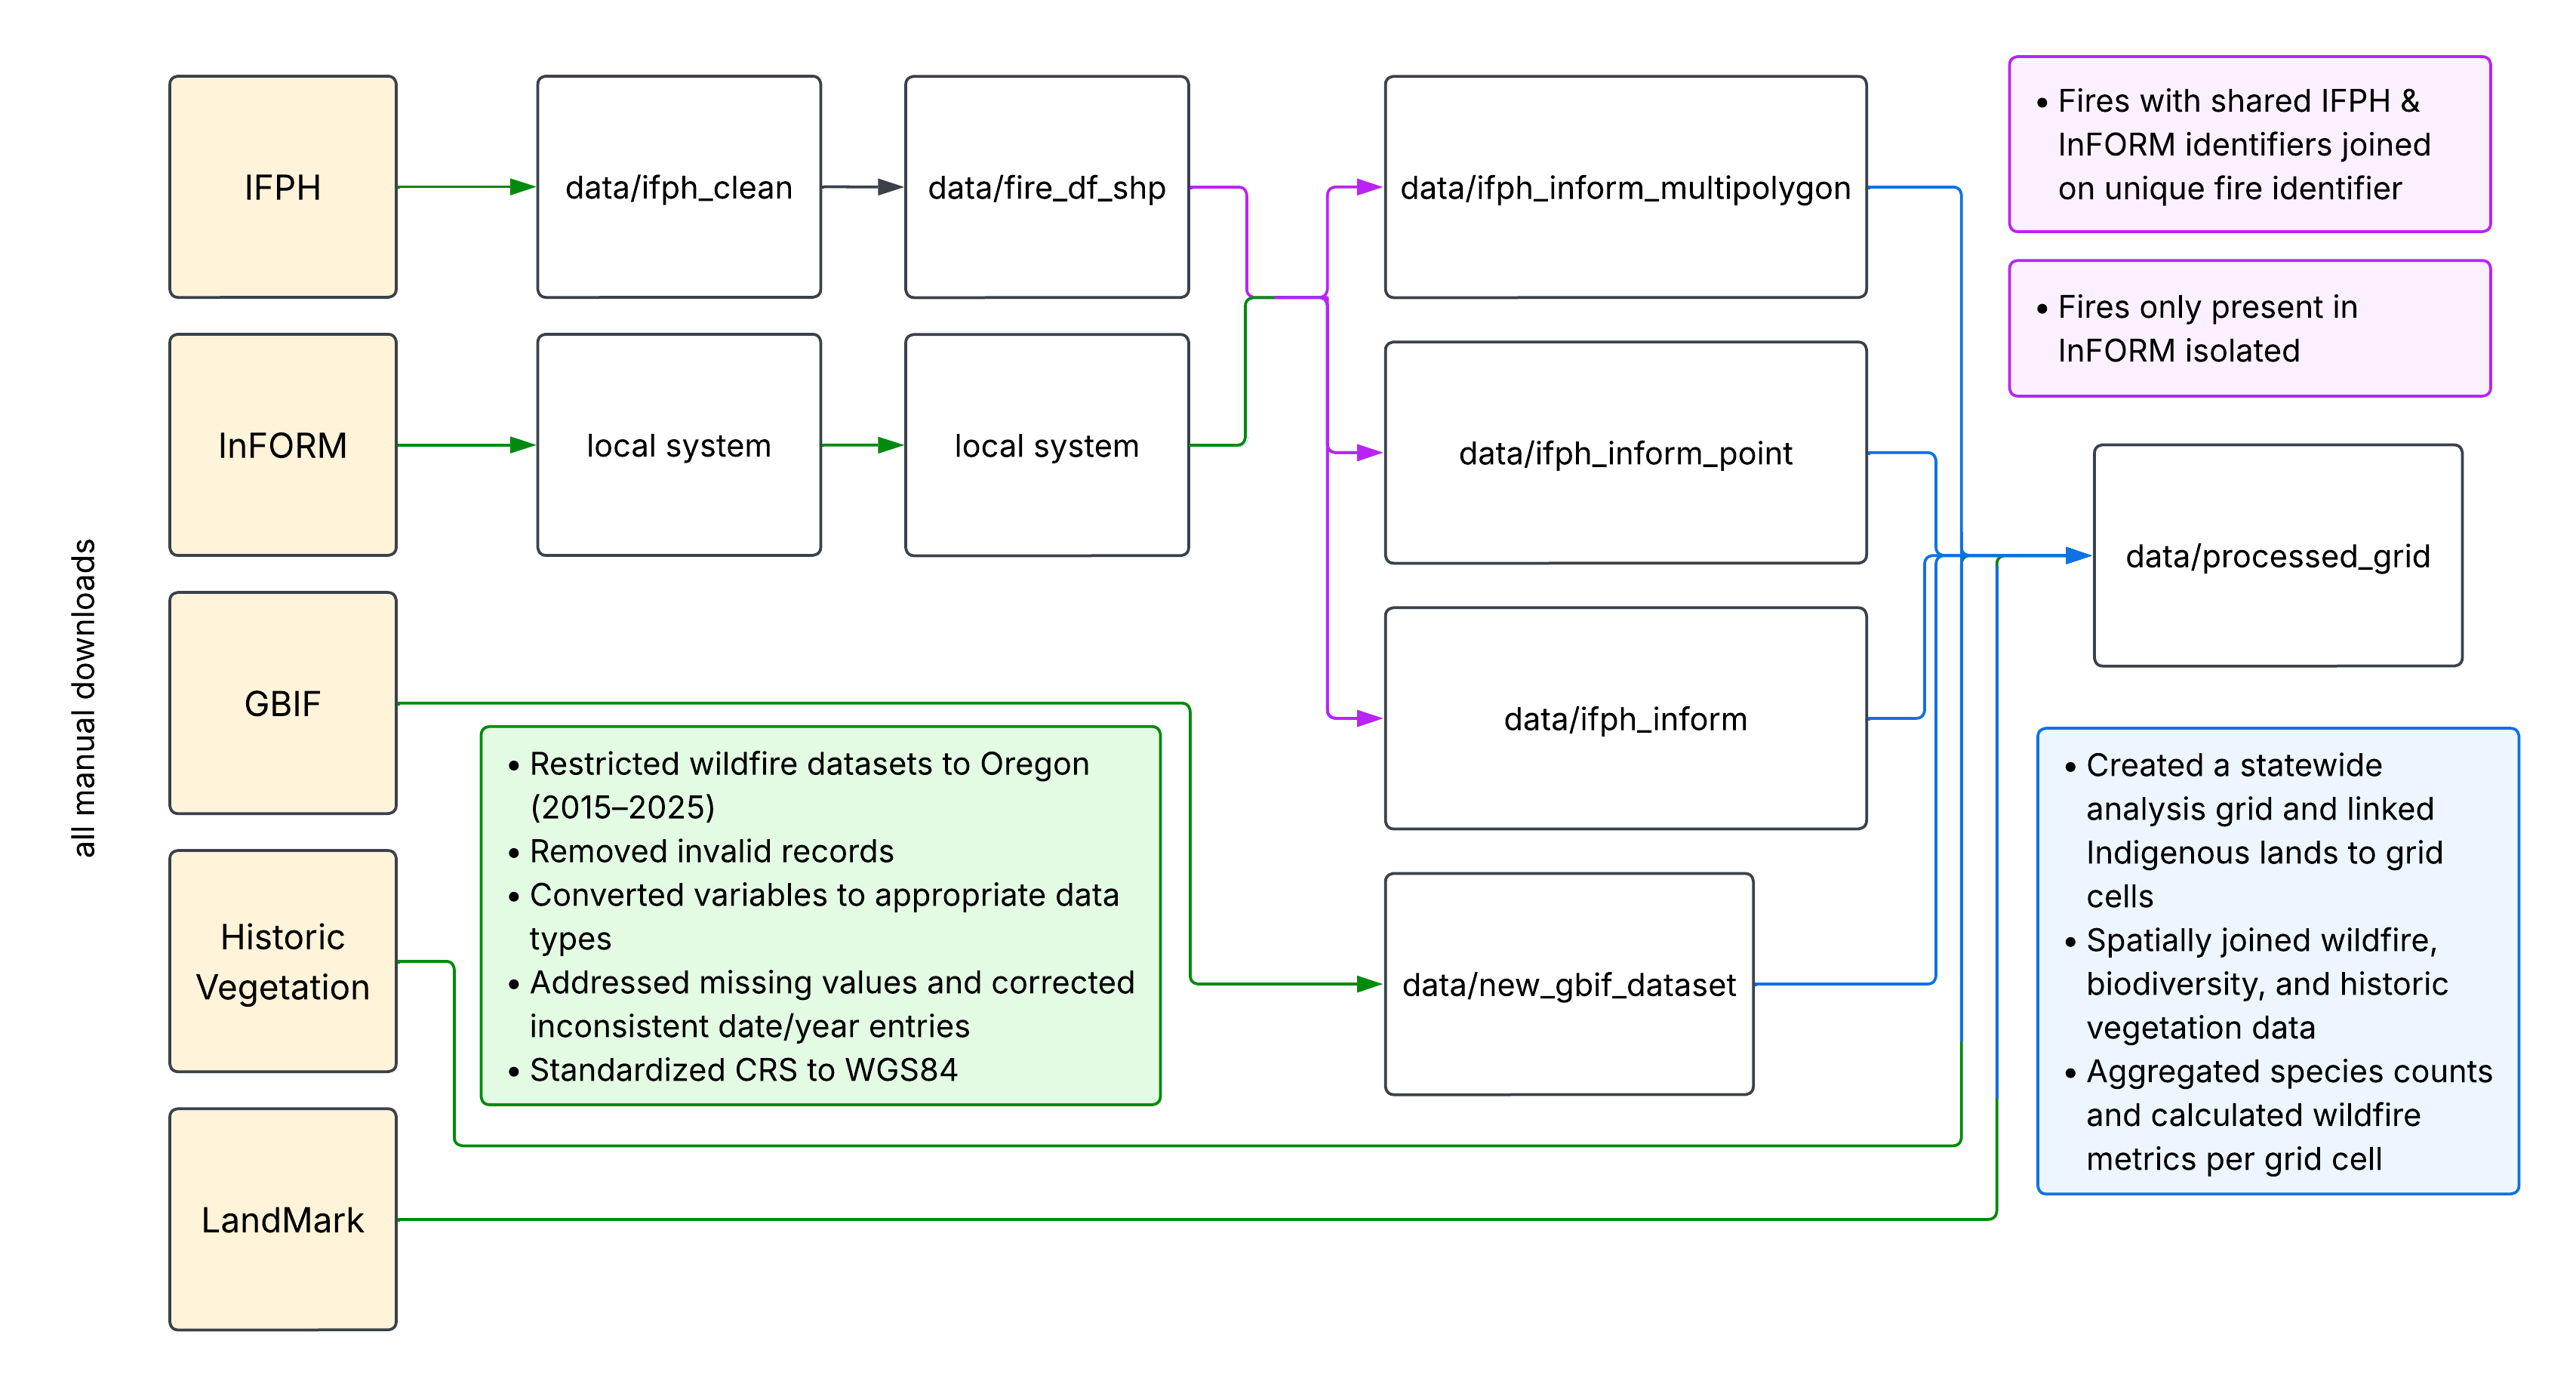
\includegraphics[keepaspectratio,alt={Diagram showing the data engineering pipeline.}]{./images/short-pipeline-capstone.png}}

}

\caption{\label{fig-pipeline}Data Engineering Pipeline}

\end{figure}%

\subsubsection{Data Cleaning and Quality
Assurance}\label{data-cleaning-and-quality-assurance}

Each dataset underwent systematic quality assessment prior to
integration. Initial inspection identified differences in variable
naming conventions, data types, coordinate reference systems, temporal
coverage, and missing values. Date fields were standardized into
consistent datetime formats, and categorical variables were recoded and
leveled where appropriate. \hspace{0pt} The IFPH and InFORM data share a
common unique fire identifier, which was used to join common fires. 817
records had matching identifiers in IFPH and InFORM; for these fires,
IFPH values were preferred when both datasets were available, including
the multipolygon geometry provided by IFPH. We excluded 866 records in
the IFPH dataset that did not have counterparts in InFORM data from
subsequent processing because they lacked the information necessary for
our analysis. Fire records present only in InFORM were spatially placed
using the provided coordinates and converted to point geometries; this
included 10,686 records in Oregon from 2015-2025. Additionally, 27,538
records in InFORM within that time span lacked coordinates and were not
included. However, these points were not necessarily within the spatial
scope, as InFORM includes records from across the United States.
\hspace{0pt} Additional work was undertaken to construct serviceable
fire-start and fire-end dates. Three fire-end variables were available
in the InFORM data (control date-time, contain date-time, and fire out
date), each with varying levels of missingness. If multiple existed, the
latest recorded date was used to represent the fire-end date. 3443
point-based InFORM and 192 combined IFPH-InFORM polygon records were
missing all three end-date variables and were therefore excluded from
fire duration analyses; however, they were still included in fire size
analyses. \hspace{0pt} Several quality control procedures were
implemented throughout preprocessing. We standardized coordinate
reference systems to WGS 84 across all spatial datasets to ensure
accurate spatial joins. We inspected variable ranges for implausible
values, removing one wildfire record with a negative burned area,
standardizing 1970-01-01 dates to NA, and correcting two years that were
off by one century (e.g., 2121 was changed to 2021). When missing, the
calendar year was imputed from the fire discovery date-time, which had
no missingness. Other missing values were evaluated on a
variable-by-variable basis, with variables exhibiting extensive or
complete missingness (e.g., discovery acres, estimated cost to date,
final acres, final fire report approved by unit, general fire behavior,
incident short description, reimbursability indicator, POO
jurisdictional parent unit, and percent contained) excluded from
downstream analyses. Rather than imputing observations, missing values
were excluded from modeling. This approach avoided introducing
artificial observations while preserving the integrity of the original
datasets.

\subsubsection{Spatial Integration and Feature
Engineering}\label{spatial-integration-and-feature-engineering}

One of the primary contributions of this project is a reproducible
spatial integration framework that combines heterogeneous datasets and
geometries into standardized analytical units. All datasets were
spatially joined using a common 5 km × 5 km analysis grid covering the
state of Oregon, created using the US National Atlas Equal Area
coordinate reference system. This grid provided a consistent spatial
resolution for summarizing wildfire records, prescribed fire occurrence,
vegetation characteristics, and Indigenous land designation. After its
creation, the grid and all other spatial datasets were converted to the
WGS 84 coordinate reference system, except InFORM and GBIF, which were
already in WGS 84.\hspace{0pt}

For each grid cell, we calculated a more representative species count by
combining GBIF occurrence records with Historic Vegetation, increasing
the plant occurrence count by one for any cell that intersected a
relevant vegetation region. This operation was performed for Ponderosa
Pine, Scouler's Willow, Oregon White Oak, Black Cottonwood, and Western
Rederar. California Blackberry and Beargrass were not included in the
Historic Vegetation dataset, which focuses on broader patterns of
dominant species, so their counts are based solely on GBIF records.
Dual-tree categories were used for Ponderosa Pine and Oregon White Oak
to include as many applicable regions as possible. Shannon Diversity
Index values were subsequently calculated using the aggregated
abundances to provide a quantitative measure of overall forest
compositional diversity.

\begin{longtable}[]{@{}
  >{\raggedright\arraybackslash}p{(\linewidth - 4\tabcolsep) * \real{0.3333}}
  >{\raggedright\arraybackslash}p{(\linewidth - 4\tabcolsep) * \real{0.3333}}
  >{\raggedright\arraybackslash}p{(\linewidth - 4\tabcolsep) * \real{0.3333}}@{}}
\caption{GBIF Species \& Oregon Historic Vegetation Region Inventory
Table.}\label{tbl-gbif-histveg-cell-inventory}\tabularnewline
\toprule\noalign{}
\begin{minipage}[b]{\linewidth}\raggedright
GBIF Species Common Name
\end{minipage} & \begin{minipage}[b]{\linewidth}\raggedright
Oregon Historic Vegetation Region(s)
\end{minipage} & \begin{minipage}[b]{\linewidth}\raggedright
Number of Cells with Designation
\end{minipage} \\
\midrule\noalign{}
\endfirsthead
\toprule\noalign{}
\begin{minipage}[b]{\linewidth}\raggedright
GBIF Species Common Name
\end{minipage} & \begin{minipage}[b]{\linewidth}\raggedright
Oregon Historic Vegetation Region(s)
\end{minipage} & \begin{minipage}[b]{\linewidth}\raggedright
Number of Cells with Designation
\end{minipage} \\
\midrule\noalign{}
\endhead
\bottomrule\noalign{}
\endlastfoot
Ponderosa Pine & Ponderosa pine, Ponderosa Pine-Lodgepole Pine, Douglas
Fir-Ponderosa Pine & 3,431 \\
Scouler's Willow & Willows & 516 \\
Oregon White Oak & White Oak Woodland, White Oak-Black Oak & 804 \\
Black Cottonwood & Black Cottonwood Riparian Woodland & 565 \\
Western Redcedar & Western Redcedar & 654 \\
Beargrass & N/A & 432 \\
California Blackberry & N/A & 932 \\
No plants recorded & N/A & 5,180 \\
\end{longtable}

\hspace{0pt}We created a binary indicator identifying whether each grid
cell intersected federally recognized Indigenous lands using LandMark.
We similarly summarized wildfire variables at the grid-cell level. These
included wildfire counts, maximum wildfire duration in hours, maximum
wildfire size in acres, wildfire size class (a factor based on the
National Wildfire Coordinating Group's size classifications), and a
count of prescribed burns with all of the above size and duration
metrics associated with them. All cells also included a list of unique
fire identifiers associated with the fires present in that cell for
manual cross-referencing with the original dataset if needed. The
resulting feature engineering process transformed over seventy thousand
individual observations into a standardized analytical dataset suitable
for comparative statistical modeling while preserving spatial
relationships among the original datasets.

In addition to the grid dataset, which included fire counts and metrics
from 2015 to 2025, we created a second dataset that aggregates fire
metrics annually. The federally recognized Indigenous land binary
variable was held constant across our time span, as land borders have
not changed during that period. Although the GBIF records had associated
dates, the vegetation columns were treated as constant because the
Historic Vegetation was not time-bound, and the resulting combined
columns were treated as proxies for general forest compositional
diversity rather than a yearly species census, given the uneven
distribution of observations. The base grid was duplicated so each grid
cell index was present for every year in the time span, and a unique row
identifier was created by combining the year and grid cell index. For
each year, the same set of fire metrics and counts were created using
only fire records from that year. Further metrics were calculated from
the time-series data, including rolling and cumulative sums of fire
counts for wildfires and prescribed burns.

\section{Ethics and Responsible Use}\label{ethics-and-responsible-use}

This project uses only publicly available ecological and geospatial
datasets and does not involve personally identifiable information or
human subjects data. Nevertheless, because several datasets concern
designated Indigenous lands, biodiversity observations, and
environmental resources, ethical data stewardship remains a central
consideration. \hspace{0pt} Analyses follow the CARE Principles for
Indigenous Data Governance (Collective Benefit, Authority to Control,
Responsibility, and Ethics) (Perreault and Goodridge 2025), recognizing
that publicly available datasets cannot fully capture Indigenous
knowledge systems, stewardship practices, or cultural relationships with
the land. Results are therefore interpreted as observational rather than
causal, avoiding broad generalizations across Indigenous nations or
deficit-based comparisons of land management practices. Findings are
reported at the landscape level to characterize ecological patterns
rather than draw cultural conclusions. \hspace{0pt} Across all datasets,
applicable licensing, attribution, and data-sharing requirements are
followed, sensitive metadata (such as observer names, recorder names,
rights-holder information, and other unnecessary identifying metadata)
are excluded from analysis and redistribution where appropriate, and
project findings are presented to support collaborative wildfire
stewardship while respecting Indigenous rights, data sovereignty, and
responsible data use.

\subsection{LandMark}\label{landmark}

The LandMark dataset provides global spatial and governance information
concerning Indigenous Peoples' and community lands, incorporating
contributed and third-party datasets describing territorial boundaries
and community-level information. Although the dataset does not contain
direct personal identifiers, it includes information about Indigenous
communities and therefore requires heightened ethical consideration. The
LandMark Terms of Service require users to protect and respect the legal
and customary rights of Indigenous Peoples and local communities and
prohibit uses that may negatively affect these communities. While
commercial-use provisions do not apply to this project, we intend to
uphold the underlying principle of equitable benefit sharing by ensuring
that findings are communicated in ways that may support the communities
represented by the data. LandMark data are generally licensed under the
Creative Commons Attribution-ShareAlike 4.0 (CC BY-SA 4.0) license,
permitting redistribution and derivative works provided appropriate
attribution is maintained, and derivatives are shared under the same
license.

\subsection{Global Biodiversity Information Facility
(GBIF)}\label{global-biodiversity-information-facility-gbif}

GBIF aggregates biodiversity occurrence records from publishers
worldwide, including species observations, museum specimens, geospatial
coordinates, observation metadata, and contributor information. Some
occurrence records include metadata identifying observers, collectors,
identifiers, rights holders, or data publisher representatives. Although
these fields are available within the raw dataset, they are not used in
this project and will be excluded from any redistributed analytical
datasets as part of a data minimization strategy. GBIF datasets are
published under standardized Creative Commons licenses (CC0, CC BY, or
CC BY-NC), with individual publishers selecting the applicable license
for their records. Accordingly, all publisher-specific licensing terms,
attribution requirements, and restrictions on commercial use will be
respected. Dataset DOIs, citations, and publisher acknowledgments will
be retained in accordance with GBIF's recommended citation practices.

\subsection{NIFC InFORM Fire Occurrence Data Records
(InFORM)}\label{nifc-inform-fire-occurrence-data-records-inform}

The NIFC InFORM Fire Occurrence Data Records (InFORM) dataset contains
operational wildfire occurrence information and does not include a
documented framework for collecting or processing personal data. No
formal license accompanies the dataset; consequently, permission should
be requested before redistribution or other uses beyond standard
research applications. In the absence of an explicit open-data license,
this project will not assume unrestricted redistribution rights, will
avoid commercial redistribution without authorization, and will preserve
source attribution and source throughout the analytical workflow.

\subsection{NIFC Interagency Wildland Fire Perimeter History
(IFPH)}\label{nifc-interagency-wildland-fire-perimeter-history-ifph}

The NIFC Interagency Wildland Fire Perimeter History (IFPH) dataset
consists of historical wildfire perimeter polygons and associated
environmental metadata. The dataset is described as being free for
strategic use, permitting its use for planning, research, and analytical
purposes. Because downstream redistribution terms are not explicitly
defined, appropriate attribution will be maintained, and any additional
federal geospatial data-use requirements will be reviewed before
publicly redistributing derivative datasets.

\subsection{Oregon Historic
Vegetation}\label{oregon-historic-vegetation}

The Oregon Historic Vegetation dataset contains polygon-based geospatial
features describing reconstructed historical vegetation communities and
associated ecological characteristics. The dataset is released under the
Creative Commons CC0 1.0 Public Domain Dedication, allowing unrestricted
reuse, redistribution, and creation of derivative works without a legal
requirement for attribution. Although attribution is not required under
the license, this project will continue to cite the dataset and document
its source for scientific transparency and reproducibility.

\section{Methods and Evaluation}\label{methods-and-evaluation}

\subsection{Research Question 1}\label{research-question-1}

\subsubsection{Methods}\label{methods}

\subsubsection{Evaluation}\label{evaluation}

\subsection{Research Question 2}\label{research-question-2}

\subsubsection{Methods}\label{methods-1}

\subsubsection{Evaluation}\label{evaluation-1}

\subsection{Research Question 3}\label{research-question-3}

\subsubsection{Methods}\label{methods-2}

\begin{longtable}[]{@{}lr@{}}
\caption{Binned fire size
categories.}\label{tbl-fire-size-bins}\tabularnewline
\toprule\noalign{}
Fire Size Category & Acres Burned \\
\midrule\noalign{}
\endfirsthead
\toprule\noalign{}
Fire Size Category & Acres Burned \\
\midrule\noalign{}
\endhead
\bottomrule\noalign{}
\endlastfoot
Small & X ≤ 0.1 \\
Medium & 0.1 \textless{} X ≤ 4.72 \\
Large & \textgreater{} 4.72 \\
\end{longtable}

\subsubsection{Evaluation}\label{evaluation-2}

\section{Results and Visualizations}\label{results-and-visualizations}

\subsection{Research Question 1}\label{research-question-1-1}

\begin{figure}

\centering{

\pandocbounded{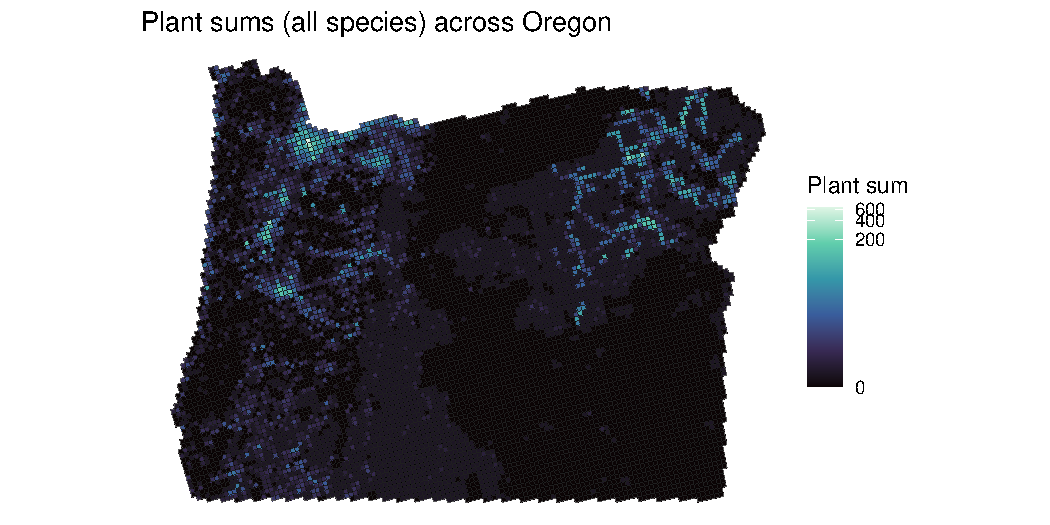
\includegraphics[keepaspectratio]{writeup_files/figure-pdf/fig-all-plants-map-1.pdf}}

}

\caption{\label{fig-all-plants-map}Plant occurrence sums.}

\end{figure}%

\subsubsection{Species-Level
Comparisons}\label{species-level-comparisons}

\begin{longtable}[]{@{}
  >{\raggedright\arraybackslash}p{(\linewidth - 8\tabcolsep) * \real{0.2000}}
  >{\raggedright\arraybackslash}p{(\linewidth - 8\tabcolsep) * \real{0.2000}}
  >{\raggedright\arraybackslash}p{(\linewidth - 8\tabcolsep) * \real{0.2000}}
  >{\raggedright\arraybackslash}p{(\linewidth - 8\tabcolsep) * \real{0.2000}}
  >{\raggedright\arraybackslash}p{(\linewidth - 8\tabcolsep) * \real{0.2000}}@{}}
\caption{Species Distribution by Indigenous land designation
status.}\label{tbl-species-dist-indigenous}\tabularnewline
\toprule\noalign{}
\begin{minipage}[b]{\linewidth}\raggedright
Plant Species
\end{minipage} & \begin{minipage}[b]{\linewidth}\raggedright
Mean Species Abundance (Non-Indigenous)
\end{minipage} & \begin{minipage}[b]{\linewidth}\raggedright
Mean Species Abundance (Indigenous)
\end{minipage} & \begin{minipage}[b]{\linewidth}\raggedright
Welch's t-test p-values
\end{minipage} & \begin{minipage}[b]{\linewidth}\raggedright
Mann-Whiteney U p-values
\end{minipage} \\
\midrule\noalign{}
\endfirsthead
\toprule\noalign{}
\begin{minipage}[b]{\linewidth}\raggedright
Plant Species
\end{minipage} & \begin{minipage}[b]{\linewidth}\raggedright
Mean Species Abundance (Non-Indigenous)
\end{minipage} & \begin{minipage}[b]{\linewidth}\raggedright
Mean Species Abundance (Indigenous)
\end{minipage} & \begin{minipage}[b]{\linewidth}\raggedright
Welch's t-test p-values
\end{minipage} & \begin{minipage}[b]{\linewidth}\raggedright
Mann-Whiteney U p-values
\end{minipage} \\
\midrule\noalign{}
\endhead
\bottomrule\noalign{}
\endlastfoot
Ponderosa Pine & 1.20487854 & 1.2257143 & 0.9450517 & 0.0001186367 \\
Scouler's Willow & 0.05751857 & 0.0400000 & 0.1785742 & 0.1699796488 \\
Oregon White Oak & 0.43896808 & 0.4000000 & 0.7547603 & 0.8492149566 \\
Black Cottonwood & 0.16181490 & 0.1171429 & 0.4764685 & 0.9087538262 \\
Western Redcedar & 0.34661715 & 0.0400000 & 7.552007e-07 &
0.0109302547 \\
Beargrass & 0.17165228 & 0.1171429 & 0.1510516 & 0.3628868174 \\
California Blackberry & 0.35555109 & 0.1657143 & 2.297990e-05 &
0.8777980018 \\
\end{longtable}

\begin{figure}

\centering{

\pandocbounded{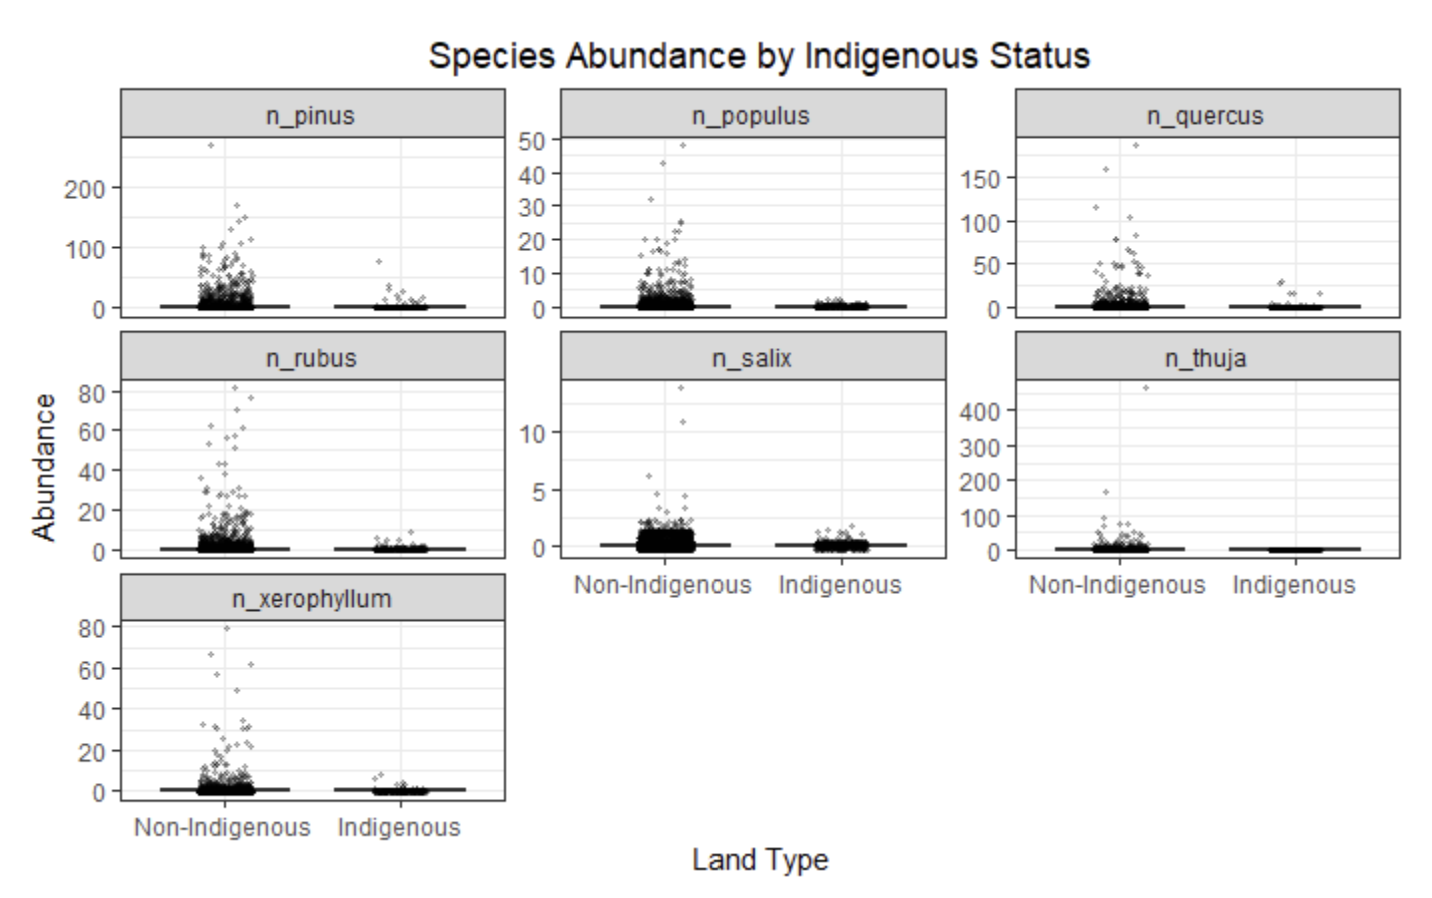
\includegraphics[keepaspectratio]{./images/species_abundance_scatterplot.png}}

}

\caption{\label{fig-species-abundance}Species abundance by Indigenous
land designation status.}

\end{figure}%

\subsubsection{Shannon Diversity}\label{shannon-diversity}

\subsubsection{Model Validation}\label{model-validation}

\begin{figure}

\centering{

\pandocbounded{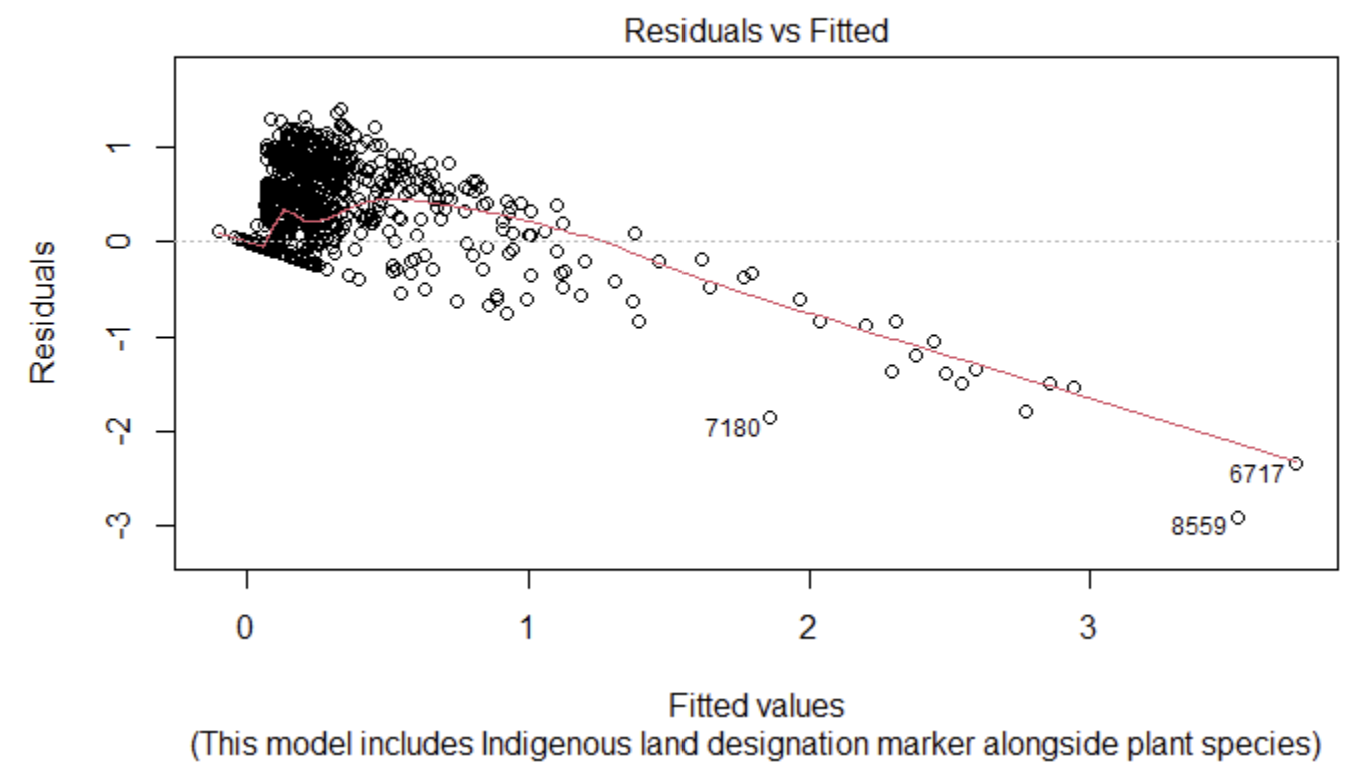
\includegraphics[keepaspectratio]{./images/species_residvfitted_plot.png}}

}

\caption{\label{fig-species-resid-fitted}Forest compositional diversity
residuals vs fitted.}

\end{figure}%

\begin{figure}

\centering{

\pandocbounded{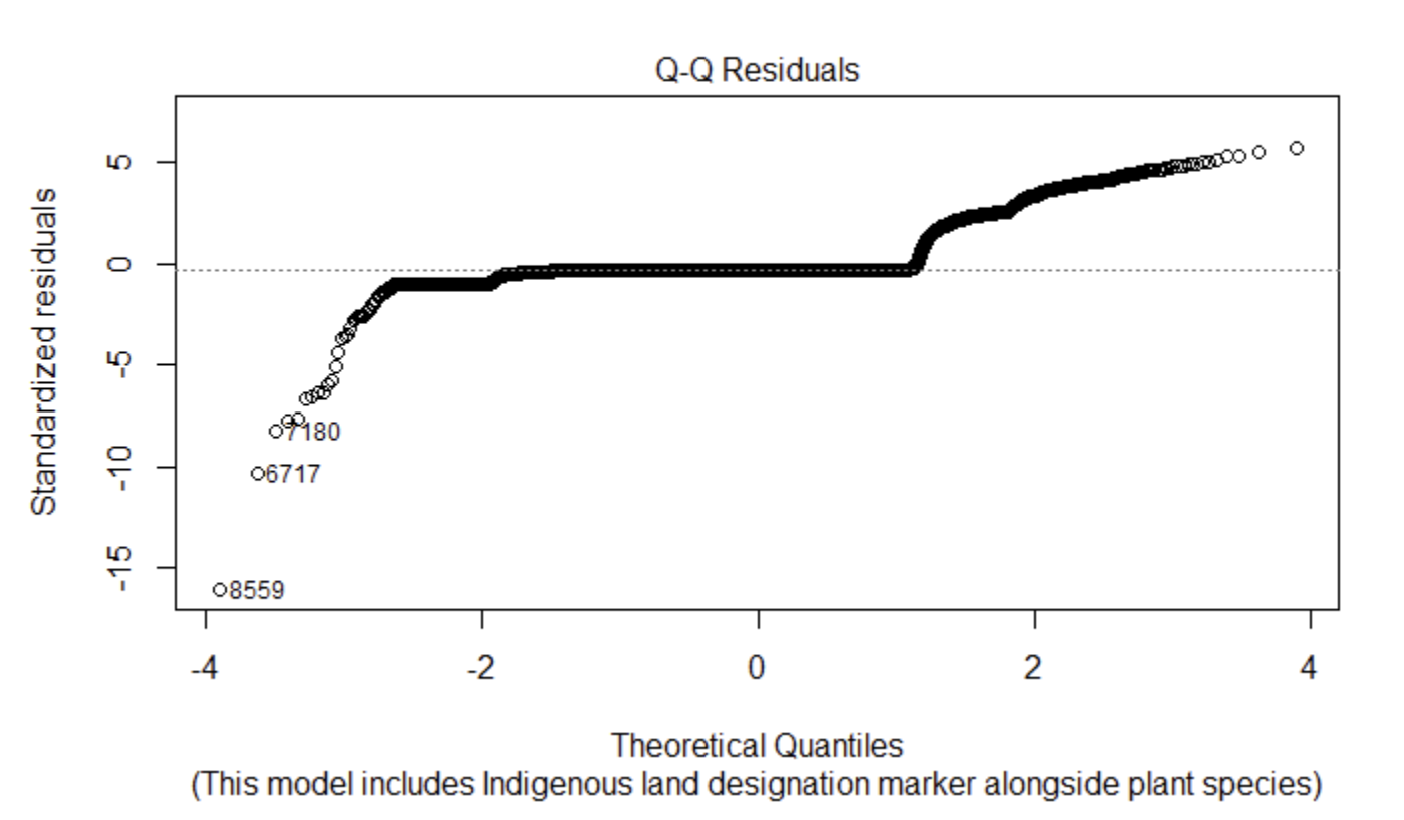
\includegraphics[keepaspectratio]{./images/species_qq_plot.png}}

}

\caption{\label{fig-species-qq}Forest compositional diversity q-q
residuals.}

\end{figure}%

\begin{figure}

\centering{

\pandocbounded{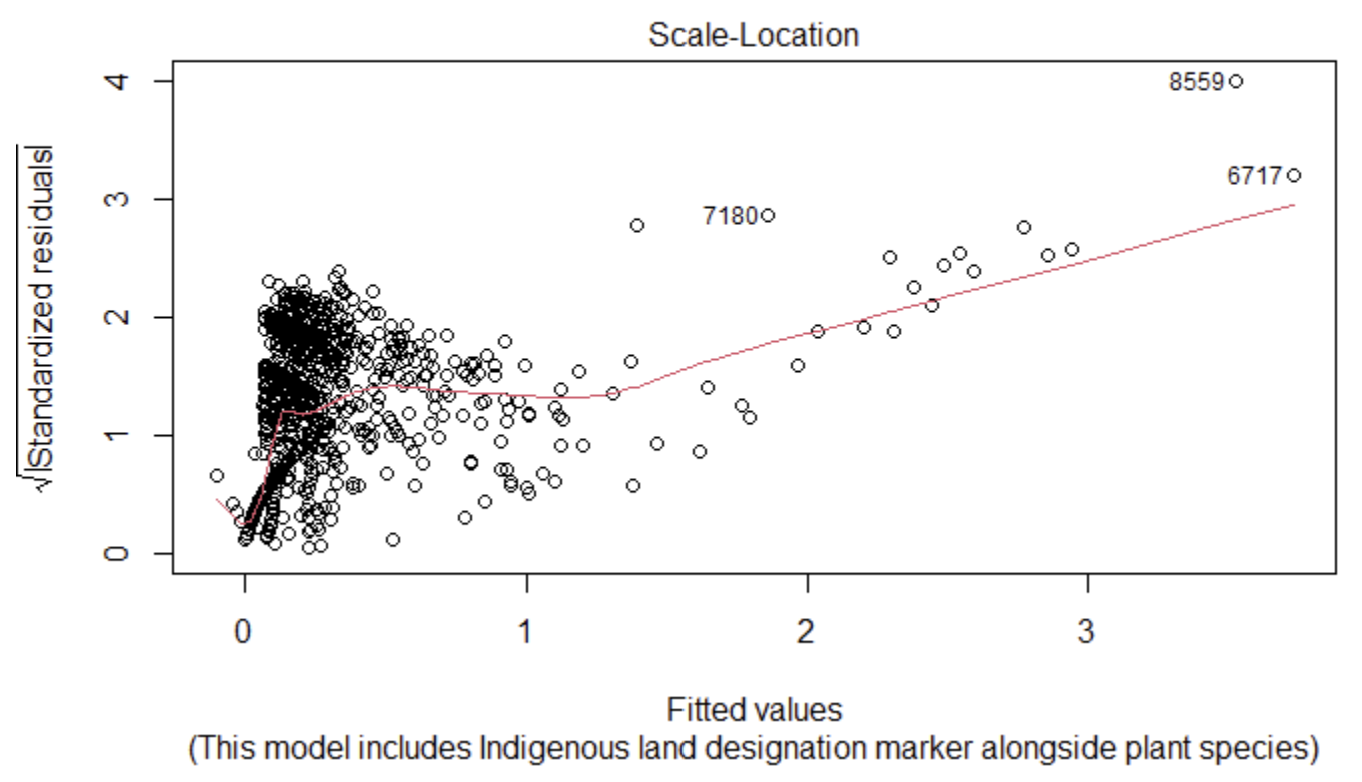
\includegraphics[keepaspectratio]{./images/species_scalelocation_plot.png}}

}

\caption{\label{fig-species-scalelocation}Forest compositional diversity
scale location.}

\end{figure}%

\begin{figure}

\centering{

\pandocbounded{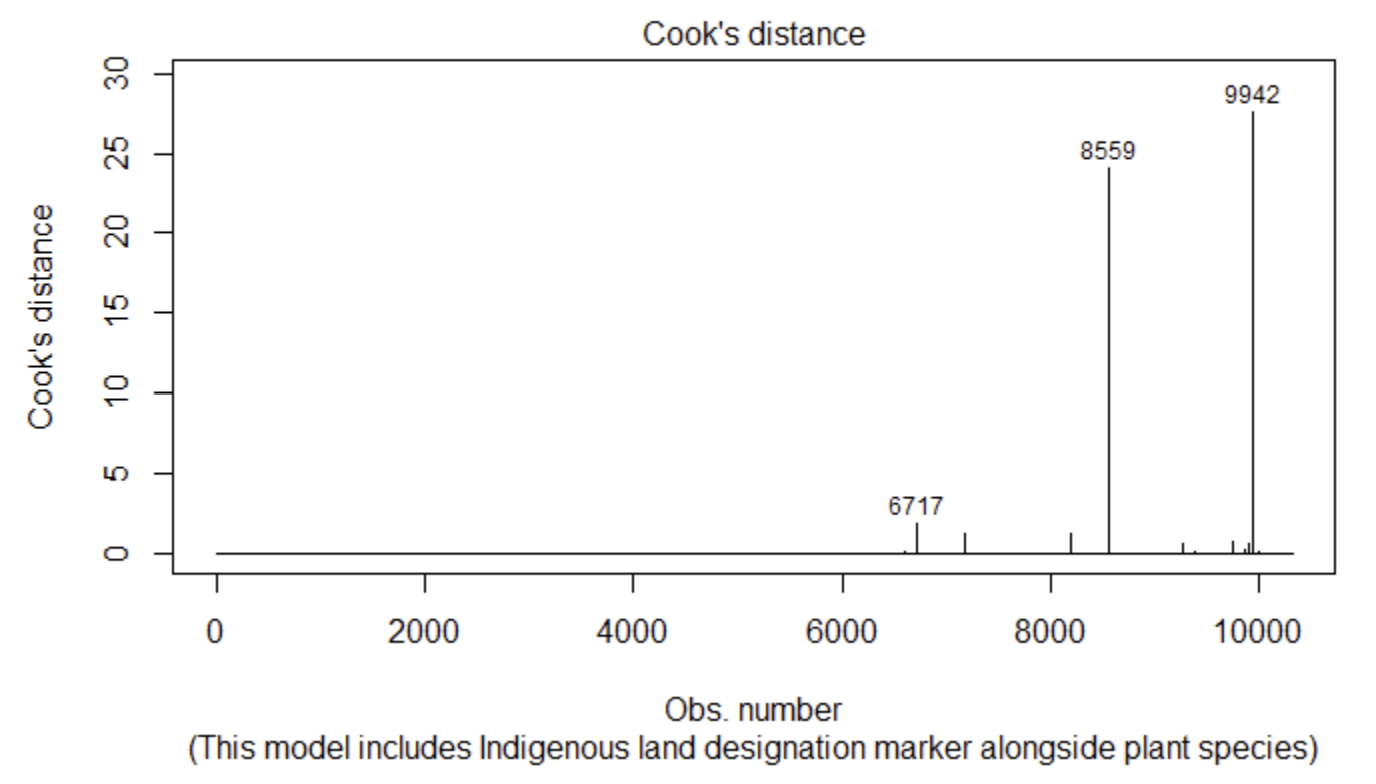
\includegraphics[keepaspectratio]{./images/species_cooks_plot.png}}

}

\caption{\label{fig-species-cooks}Forest compositional diversity Cook's
distance.}

\end{figure}%

\subsection{Research Question 2}\label{research-question-2-1}

\subsubsection{Maximum Acres Burned Across Indigenous Land
Categories}\label{maximum-acres-burned-across-indigenous-land-categories}

\begin{figure}

\centering{

\pandocbounded{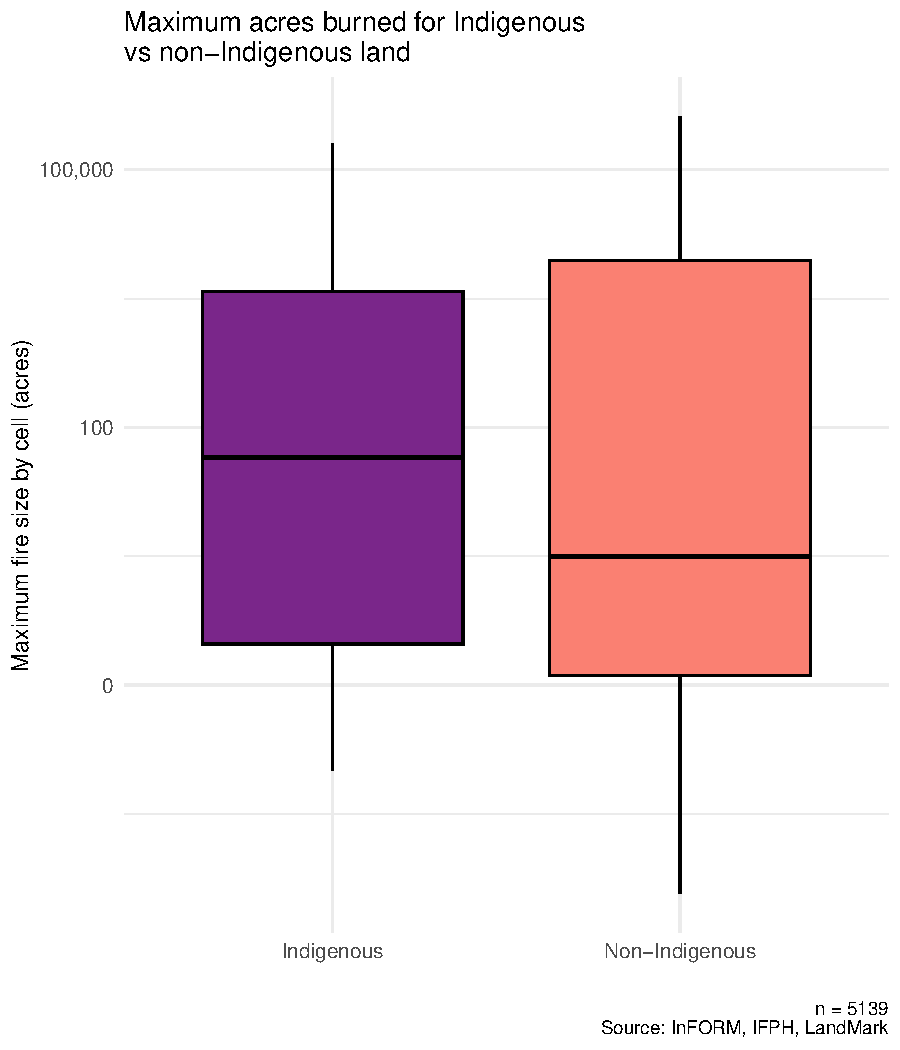
\includegraphics[keepaspectratio]{writeup_files/figure-pdf/fig-max-acres-indigenous-1.pdf}}

}

\caption{\label{fig-max-acres-indigenous}Maximum acres burned across
land designation}

\end{figure}%

{

\begin{longtable}[]{@{}lr@{}}

\caption{\label{tbl-indigenous-n-acres}Sample sizes for maximum fire
size in Indigenous and non-Indigenous designated cells.}

\tabularnewline

\toprule\noalign{}
Indigenous Status & Number of Cells \\
\midrule\noalign{}
\endhead
\bottomrule\noalign{}
\endlastfoot
Non-Indigenous & 4913 \\
Indigenous & 226 \\

\end{longtable}

}

\subsubsection{Maximum Fire Duration Across Indigenous Land
Categories}\label{maximum-fire-duration-across-indigenous-land-categories}

\begin{figure}

\centering{

\pandocbounded{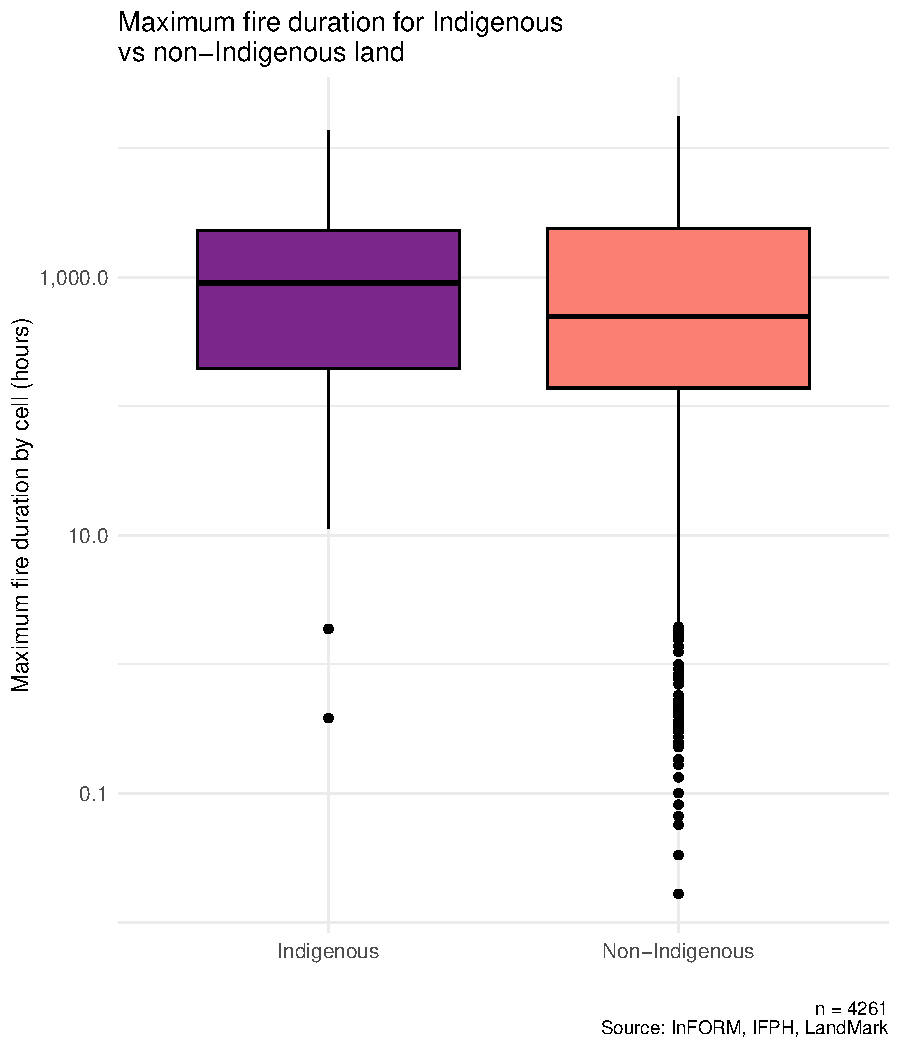
\includegraphics[keepaspectratio]{writeup_files/figure-pdf/fig-max-duration-indigenous-1.pdf}}

}

\caption{\label{fig-max-duration-indigenous}Maximum fire duration across
land designation.}

\end{figure}%

{

\begin{longtable}[]{@{}lr@{}}

\caption{\label{tbl-indigenous-n-duration}Sample sizes for maximum fire
duration in Indigenous and non-Indigenous designated cells.}

\tabularnewline

\toprule\noalign{}
Indigenous Status & Number of Cells \\
\midrule\noalign{}
\endhead
\bottomrule\noalign{}
\endlastfoot
Non-Indigenous & 4100 \\
Indigenous & 161 \\

\end{longtable}

}

\subsection{Research Question 3}\label{research-question-3-1}

\subsubsection{Comparison of Means and
Distribution}\label{comparison-of-means-and-distribution}

\begin{figure}

\centering{

\pandocbounded{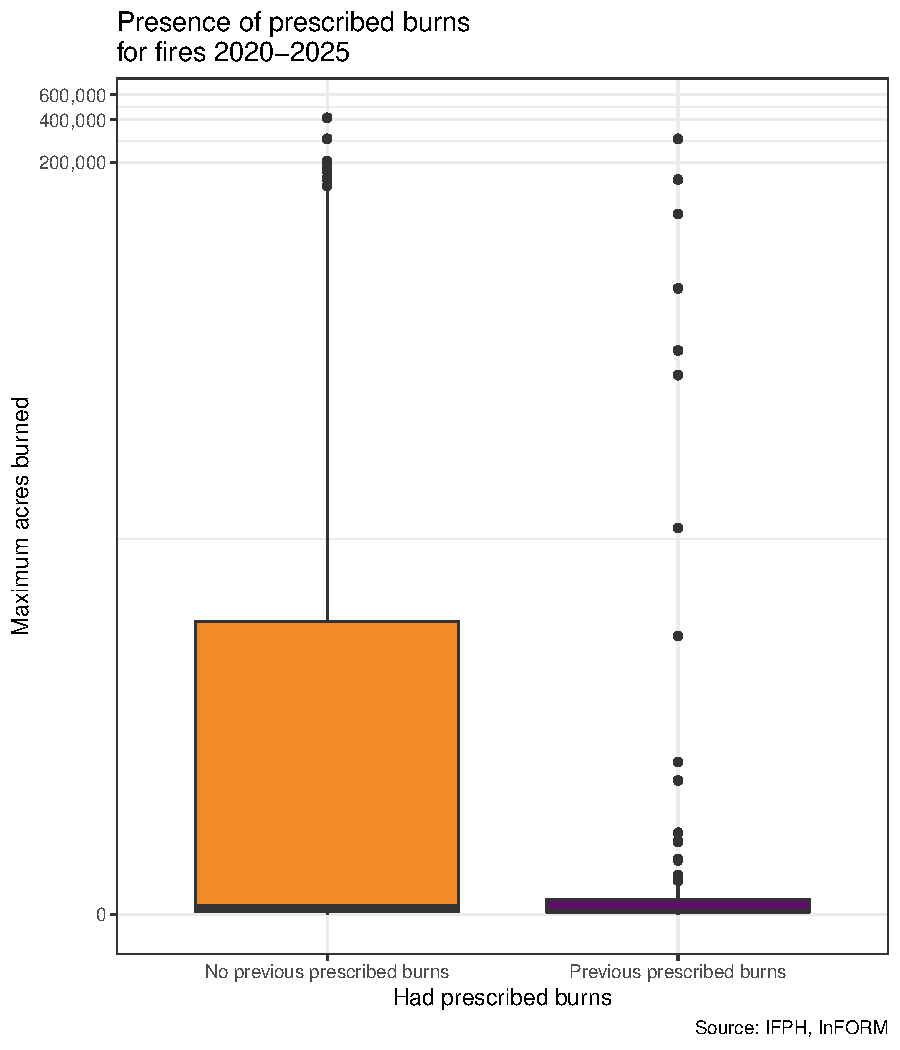
\includegraphics[keepaspectratio]{writeup_files/figure-pdf/fig-rx-acres-1.pdf}}

}

\caption{\label{fig-rx-acres}Distribution of fire size between cells
that have or have not previously had prescribed burns.}

\end{figure}%

\begin{figure}

\centering{

\pandocbounded{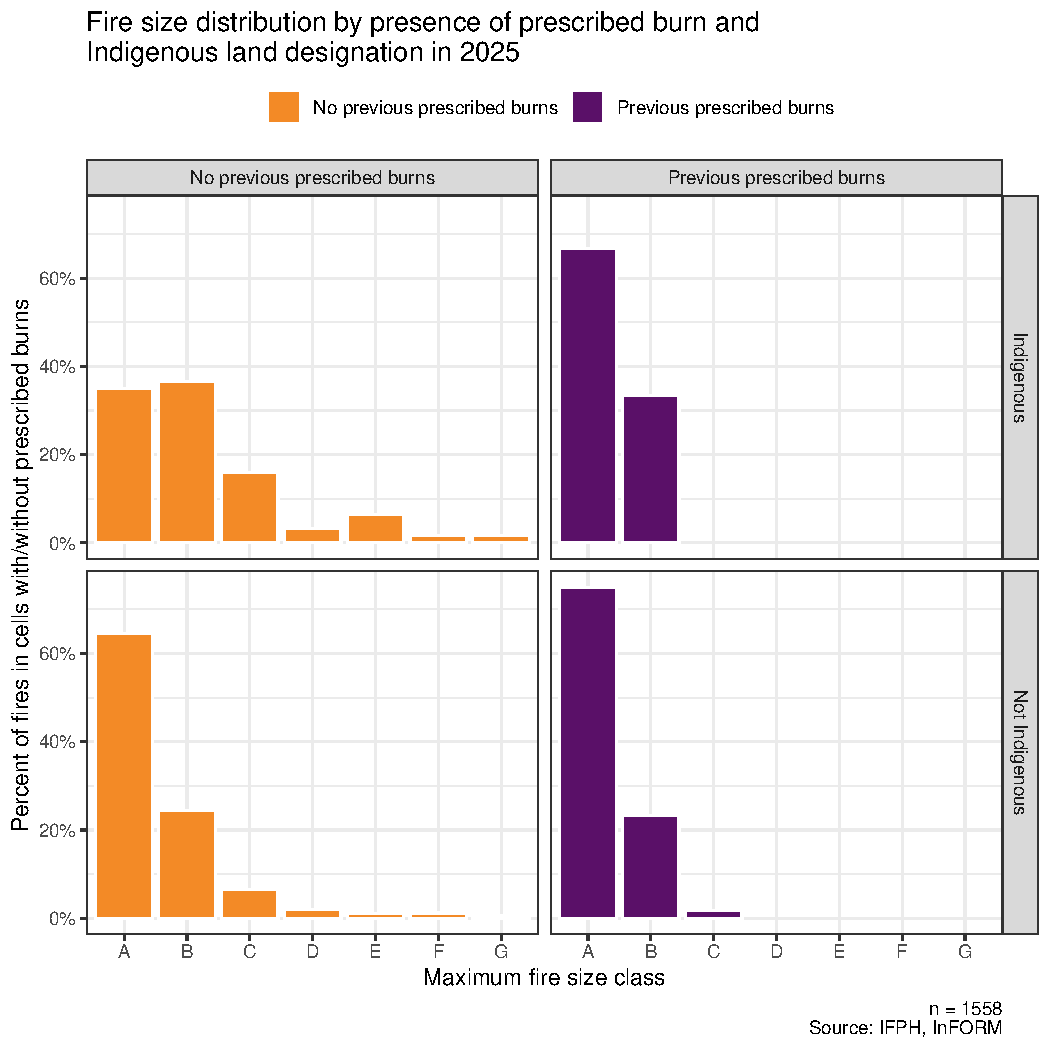
\includegraphics[keepaspectratio]{writeup_files/figure-pdf/fig-rx-indigenous-size-2025-1.pdf}}

}

\caption{\label{fig-rx-indigenous-size-2025}Fire size distribution by
the presence of prescribed burn and Indigenous land designation status
in 2025.}

\end{figure}%

{

\begin{longtable}[]{@{}llr@{}}

\caption{\label{tbl-rx-indigenous-size-2025}Sample sizes for maximum
fire size class in Indigenous and non-Indigenous designated cells with
and without previous prescribed burns in 2025.}

\tabularnewline

\toprule\noalign{}
Indigenous Status & Prescribed Burn & Number of Cells \\
\midrule\noalign{}
\endhead
\bottomrule\noalign{}
\endlastfoot
Indigenous & No previous prescribed burns & 63 \\
Indigenous & Previous prescribed burns & 6 \\
Not Indigenous & No previous prescribed burns & 1433 \\
Not Indigenous & Previous prescribed burns & 56 \\

\end{longtable}

}

\begin{figure}

\centering{

\pandocbounded{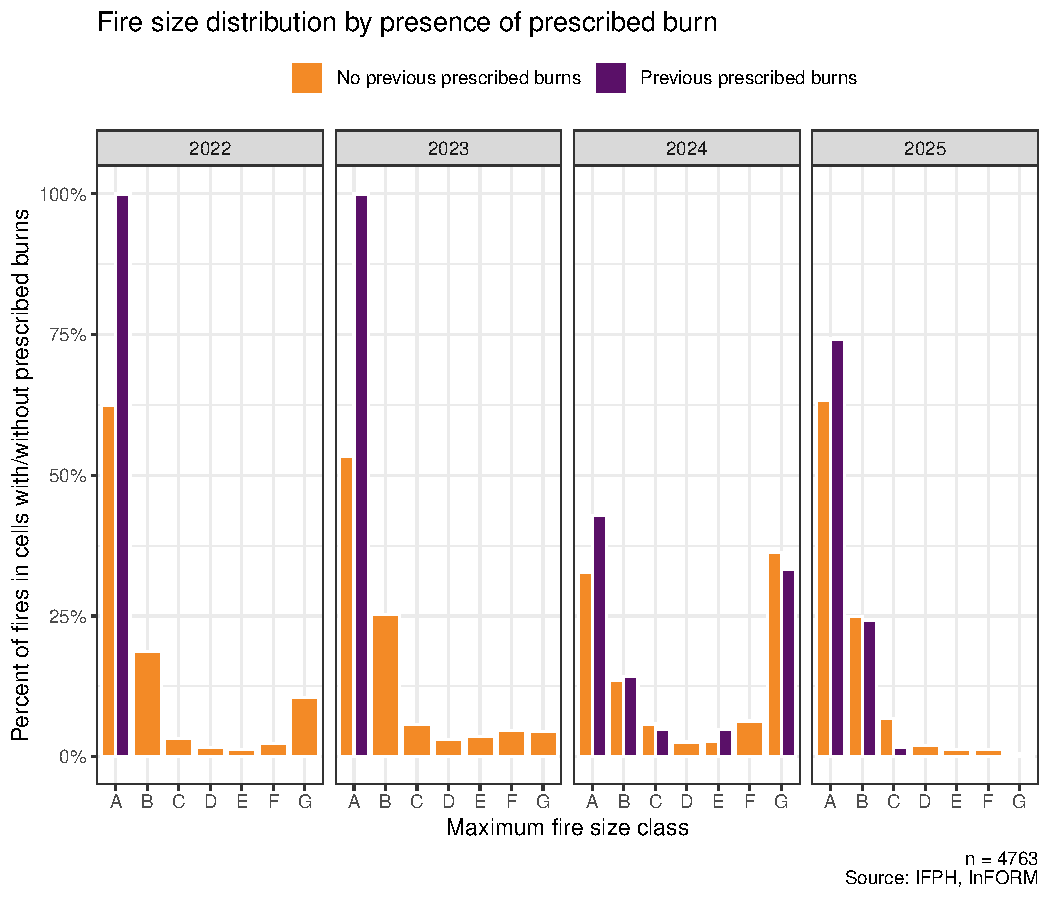
\includegraphics[keepaspectratio]{writeup_files/figure-pdf/fig-rx-annual-size-class-1.pdf}}

}

\caption{\label{fig-rx-annual-size-class}Fire class distribution by
presence of previous prescribed burn over time.}

\end{figure}%

{

\begin{longtable}[]{@{}rlr@{}}

\caption{\label{tbl-rx-size-class-annual}Sample sizes for maximum fire
size class in cells with and without previous prescribed burns
2022-2025.}

\tabularnewline

\toprule\noalign{}
Year & Prescribed Burn & Number of Cells \\
\midrule\noalign{}
\endhead
\bottomrule\noalign{}
\endlastfoot
2022 & No previous prescribed burns & 949 \\
2022 & Previous prescribed burns & 2 \\
2023 & No previous prescribed burns & 763 \\
2023 & Previous prescribed burns & 1 \\
2024 & No previous prescribed burns & 1469 \\
2024 & Previous prescribed burns & 21 \\
2025 & No previous prescribed burns & 1496 \\
2025 & Previous prescribed burns & 62 \\

\end{longtable}

}

\begin{longtable}[]{@{}lr@{}}
\caption{Size Class of Fire by Acres
Burned}\label{tbl-size-class}\tabularnewline
\toprule\noalign{}
Fire Class Category & Acres Burned \\
\midrule\noalign{}
\endfirsthead
\toprule\noalign{}
Fire Class Category & Acres Burned \\
\midrule\noalign{}
\endhead
\bottomrule\noalign{}
\endlastfoot
Class A & ≤ 0.25 acres \\
Class B & 0.25 \textless{} X ≤ 10 acres \\
Class C & 10 ≤ X \textless{} 100 acres \\
Class D & 100 ≤ X \textless{} 300 acres \\
Class E & 300 ≤ X \textless{} 1,000 acres \\
Class F & 1,000 ≤ X \textless{} 5,000 acres \\
Class G & ≥ 5,000 acres \\
\end{longtable}

\subsubsection{Modeling}\label{modeling}

\begin{figure}

\centering{

\pandocbounded{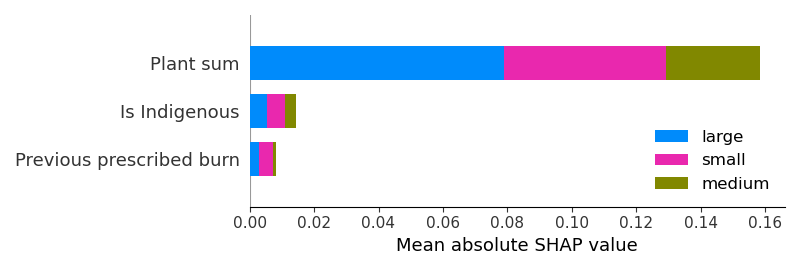
\includegraphics[keepaspectratio]{./images/shap_summary_ndgn_plnt_rx.png}}

}

\caption{\label{fig-shap-summary}SHAP values for the Random Forest
classifier with Indigenous designation, previous prescribed burn, and
plant sum.}

\end{figure}%

\begin{figure}

\centering{

\pandocbounded{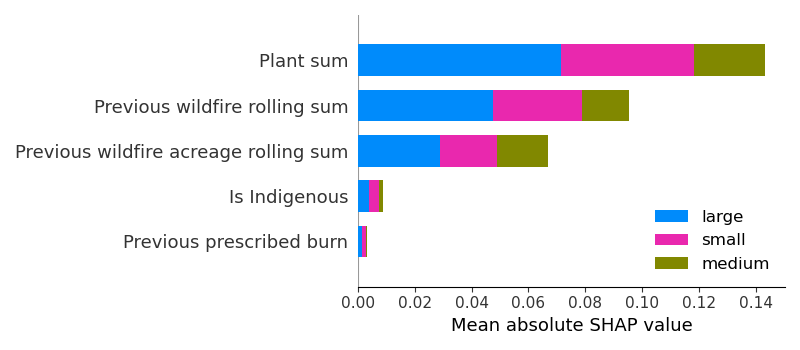
\includegraphics[keepaspectratio]{./images/shap_summary_ndgn_plnt_rx_wf.png}}

}

\caption{\label{fig-shap-summary-wf}SHAP values for the Random Forest
classifier with wildfire metrics.}

\end{figure}%

\begin{figure}

\centering{

\pandocbounded{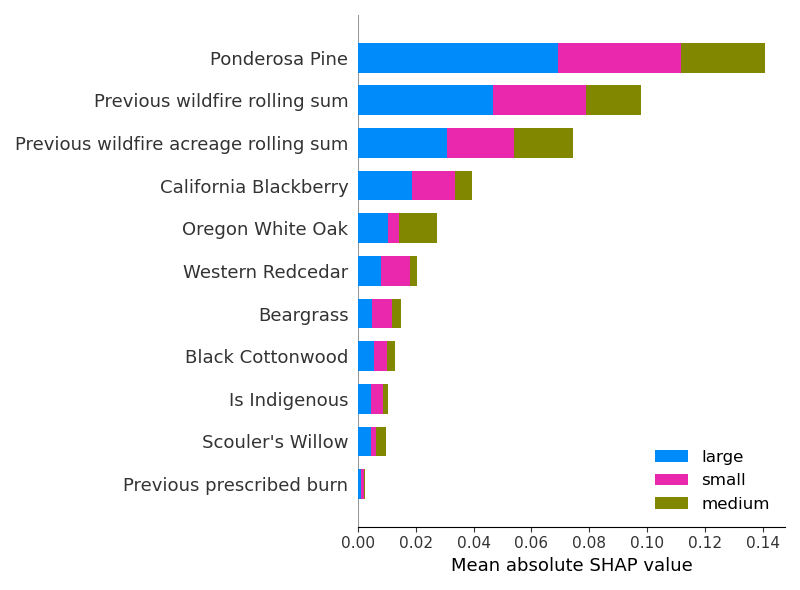
\includegraphics[keepaspectratio]{./images/shap_summary_ndgn_plnt_rx_wf_p.png}}

}

\caption{\label{fig-shap-summary-wf-p}SHAP values for the Random Forest
classifier with all plant species counts included separately.}

\end{figure}%

\begin{figure}

\centering{

\pandocbounded{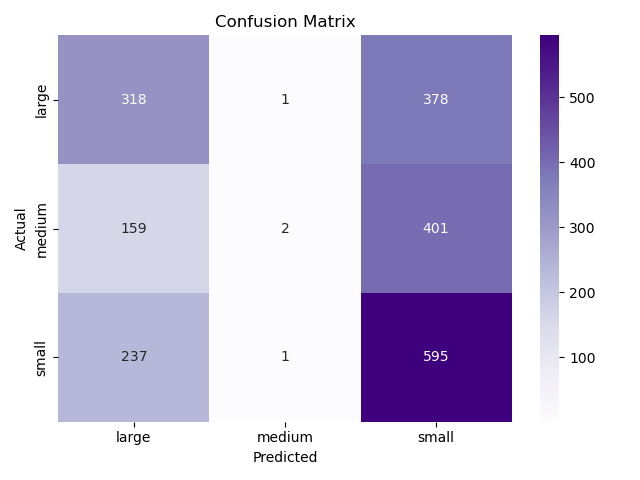
\includegraphics[keepaspectratio]{./images/conf_matrix_ndgn_plnt_rx.png}}

}

\caption{\label{fig-conf-matrix}Confusion matrix for the Random Forest
classifier with Indigenous designation, previous prescribed burn, and
plant sum.}

\end{figure}%

\begin{figure}

\centering{

\pandocbounded{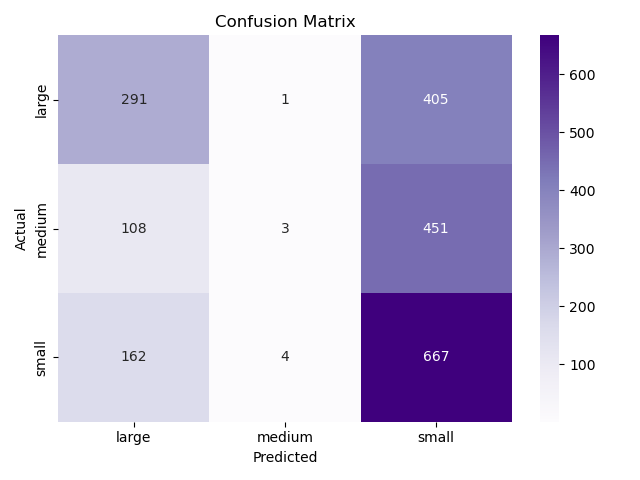
\includegraphics[keepaspectratio]{./images/conf_matrix_ndgn_plnt_rx_wf.png}}

}

\caption{\label{fig-conf-matrix-wf}Confusion matrix for the Random
Forest classifier with wildfire metrics.}

\end{figure}%

\begin{figure}

\centering{

\pandocbounded{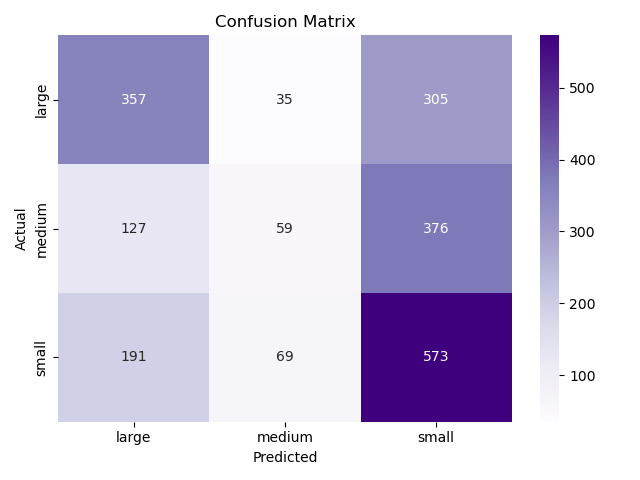
\includegraphics[keepaspectratio]{./images/conf_matrix_ndgn_plnt_rx_wf_p.png}}

}

\caption{\label{fig-conf-matrix-wf-p}Confusion matrix for the Random
Forest classifier with all plant species counts included separately.}

\end{figure}%

\section{Discussion, Limitations, and Future
Work}\label{discussion-limitations-and-future-work}

\subsection{Discussion}\label{discussion}

\subsection{Limitations}\label{limitations}

\begin{figure}

\centering{

\pandocbounded{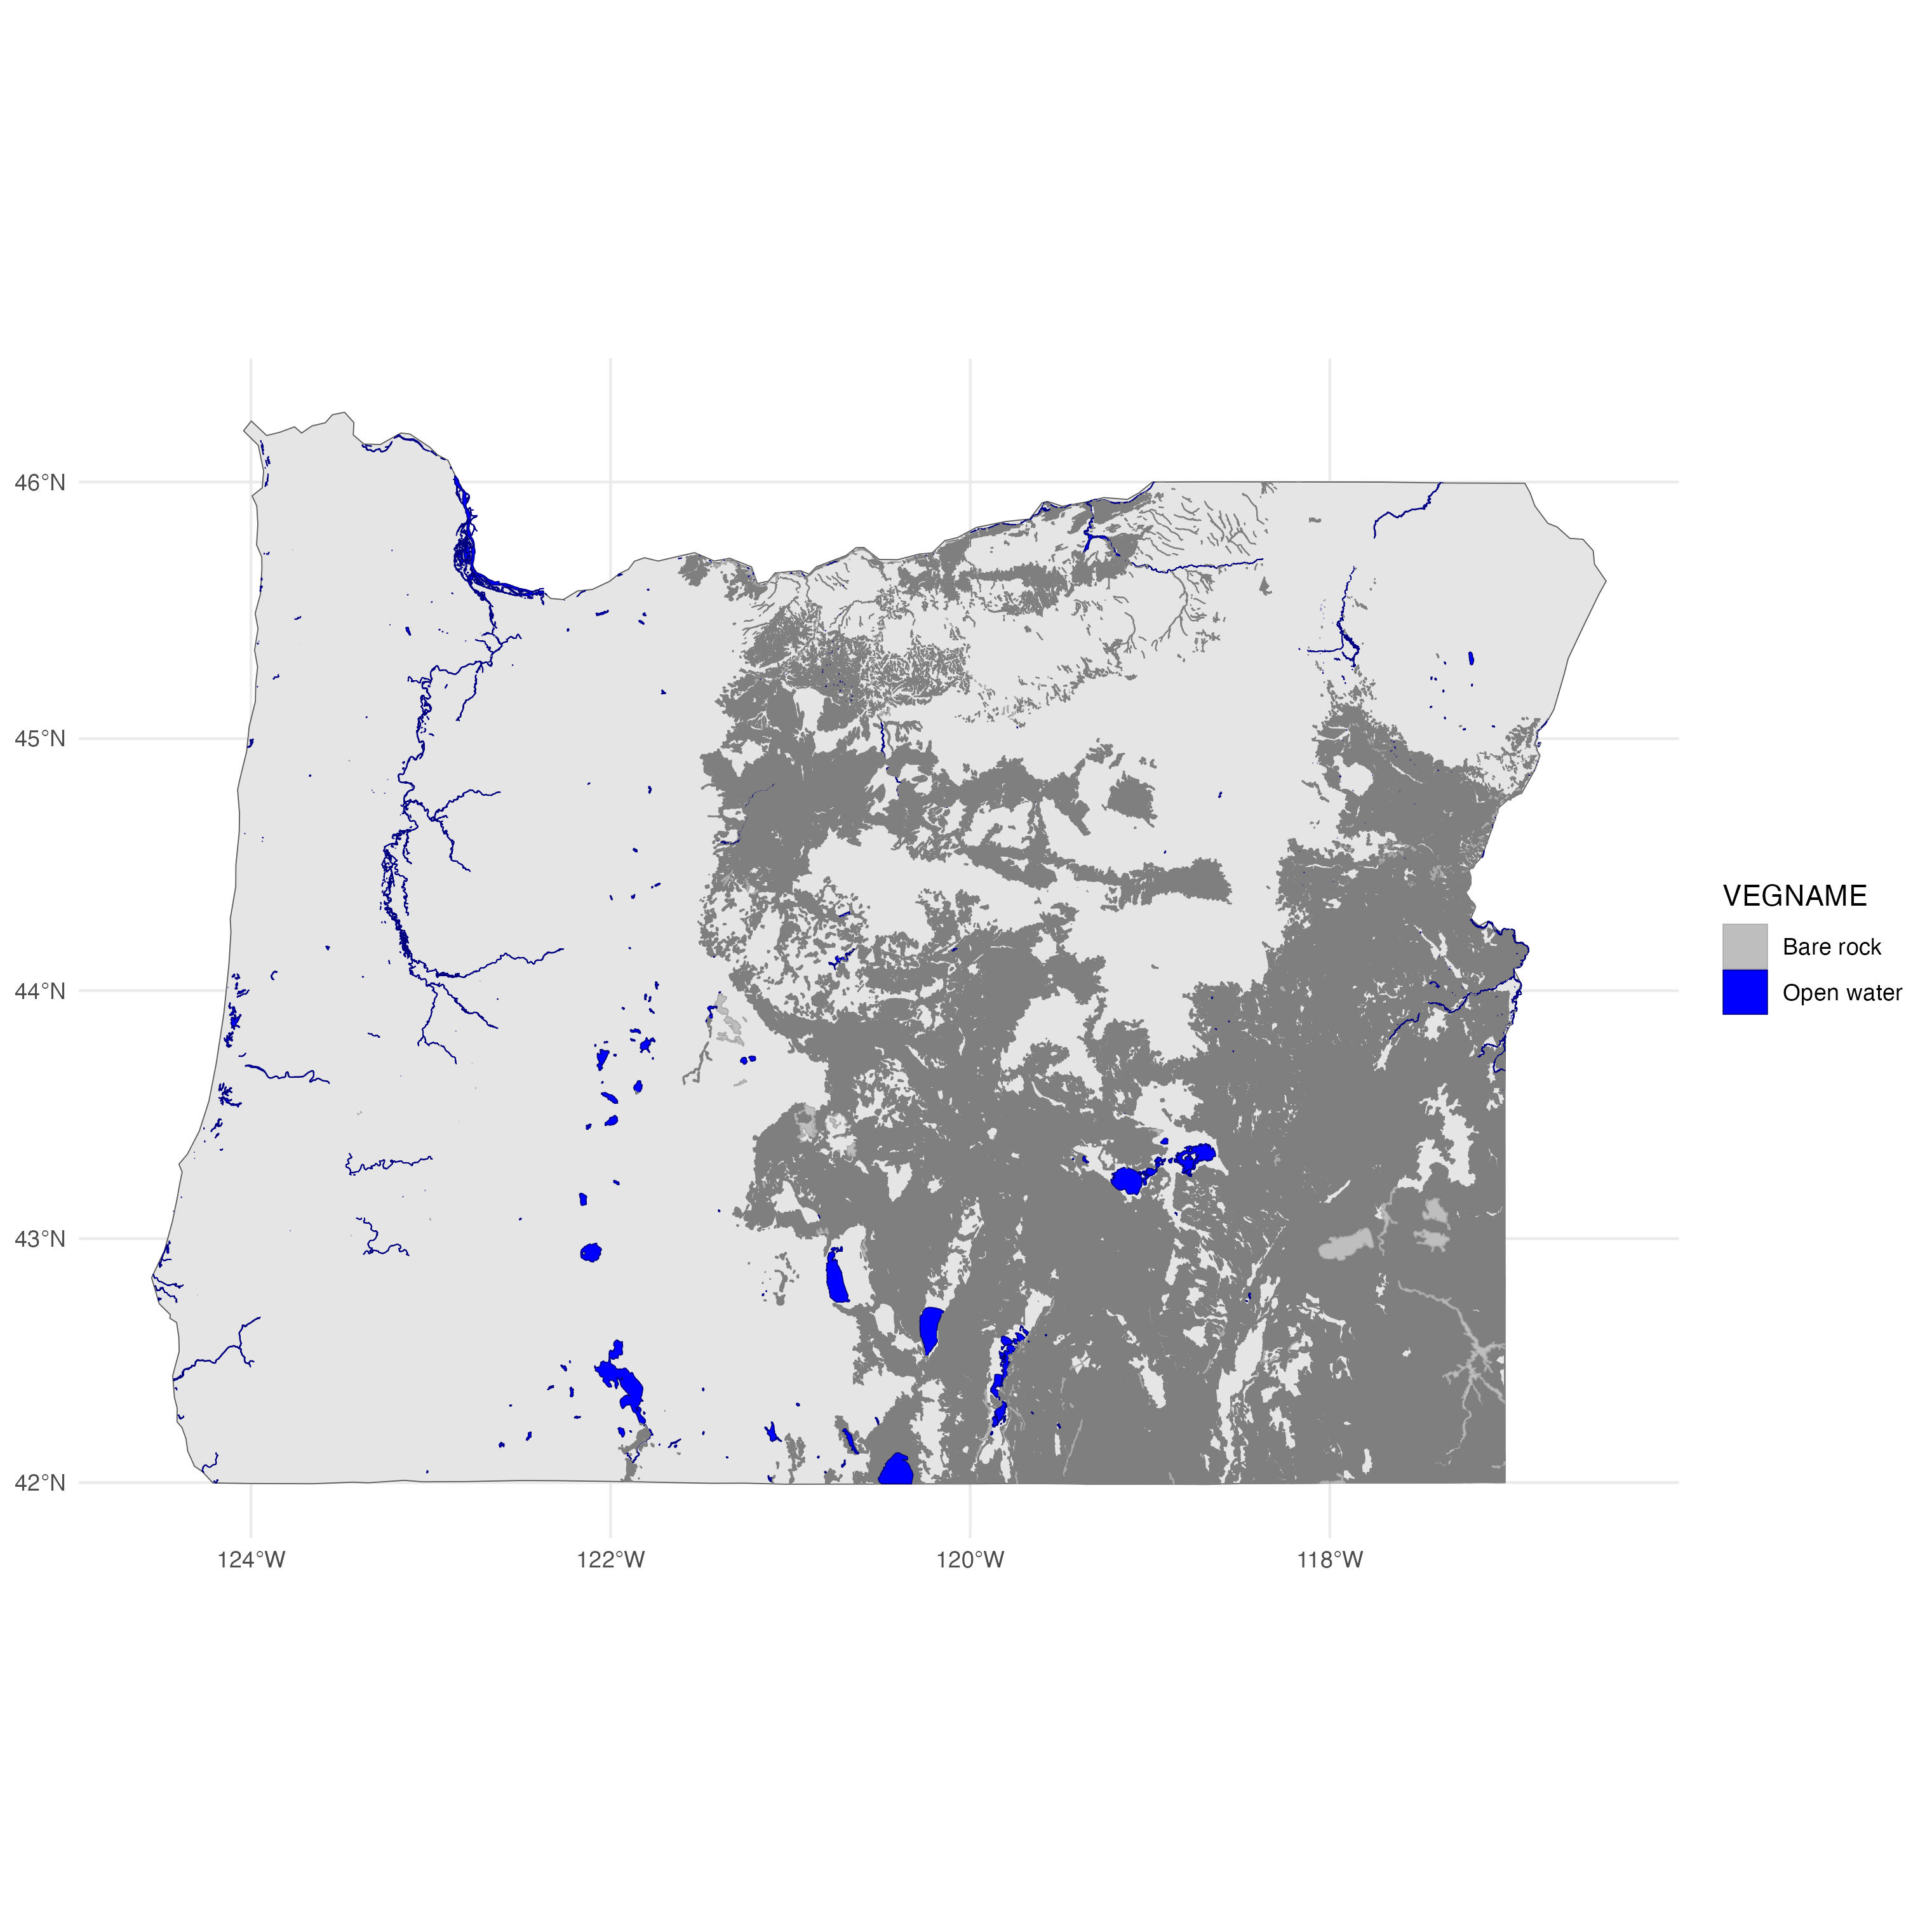
\includegraphics[keepaspectratio]{./images/noplant_plt.jpeg}}

}

\caption{\label{fig-no-plant-map}Historical Non-Vegetation Boundaries
Map}

\end{figure}%

\subsection{Future Work}\label{future-work}

\section{Conclusions and
Recommendations}\label{conclusions-and-recommendations}

\section{Reproducibility and
References}\label{reproducibility-and-references}

\textbf{Reproduce main results:}

\begin{Shaded}
\begin{Highlighting}[]
\BuiltInTok{cd}\NormalTok{ your{-}repo}
\ExtensionTok{quarto}\NormalTok{ render deliverables/M4{-}writeup{-}draft/writeup.qmd}
\end{Highlighting}
\end{Shaded}

\section{References}\label{references}

\protect\phantomsection\label{refs}
\begin{CSLReferences}{1}{1}
\bibitem[\citeproctext]{ref-abatzoglou2016}
Abatzoglou, J. T., and A. P. Willams. 2016. {``Impact of Anthropogenic
Climate Change on Wildfire Across Western US Forests \textbar{} Pnas.''}
\emph{Proceedings of the National Academy of Sciences of the United
States of America}.
\url{https://www.pnas.org/doi/10.1073/pnas.1607171113}.

\bibitem[\citeproctext]{ref-acker2024}
Acker, L. 2016-10-28. {``Oregon's Record-Breaking 2024 Fire Season Is
Finally over - Oregonlive.com.''} \emph{Oregon Live}, 2016-10-28.
\url{https://www.pnas.org/doi/10.1073/pnas.1607171113}.

\bibitem[\citeproctext]{ref-osu2019}
{``Black Cottonwood.''} 2019. \emph{College of Agricultural Sciences},
September 20.
\url{https://horticulture.oregonstate.edu/oregon-vegetables/black-cottonwood\#}.

\bibitem[\citeproctext]{ref-coughlan2024}
Coughlan, M. R., J. D. Johnston, K. M. Derr, D. G. Lewis, and B. R.
Johnson. 2024. {``Pre-Contact Indigenous Fire Stewardship: A Research
Framework and Application to a Pacific Northwest Temperate
Rainforest.''} \emph{Front. Environ. Archaeol.}, ahead of print.
\url{https://doi.org/10.3389/fearc.2024.1347571}.

\bibitem[\citeproctext]{ref-coughlan2023}
Coughlan, M., N. Serio, H. Loeb, D. Lewis, and S. Thompson. 2023.
{``Indigenous Fire Stewardship for Fire Management and Ecological
Restoration in the Pacific Northwest Ecosystem Workforce Program.''}
\emph{Northwest Fire Science Consortium}.
\url{https://www.nwfirescience.org/sites/default/files/publications/SynthesisReport_IFS_Full_Accessible_oct30.pdf}.

\bibitem[\citeproctext]{ref-coughlannd}
Coughlan, M., N. Serio, H. Loeb, D. Lewis, and S. Thompson. n.d.
\emph{Ndigenous Fire Stewardship for Fire Management and Ecological
Restoration in the Pacific Northwest Ecosystem Workforce Program}. n.d.
\url{https://www.nwfirescience.org/sites/default/files/publications/SynthesisReport_IFS_Full_Accessible_oct30.pdf}.

\bibitem[\citeproctext]{ref-fryer2018}
Fryer, J. L. n.d. {``Pinus Ponderosa Var. Benthamiana, p. Ponderosa Var.
Ponderosa, Pacific Ponderosa Pine, Columbia Ponderosa Pine.''} \emph{US
Forest Service Research and Development}.
\url{https://research.fs.usda.gov/feis/species-reviews/pinponp}.

\bibitem[\citeproctext]{ref-gbif}
\emph{GBIF Occurrence Download}. 2026. GBIF.org.
\url{https://doi.org/10.15468/dl.a9m8pz}.

\bibitem[\citeproctext]{ref-gleason2025}
Gleason, S. 2025. {``Tribes Lead the Way in Forest Resilience.''}
\emph{The Washington State Standard}.
\url{https://washingtonstatestandard.com/2025/09/25/tribes-lead-the-way-in-forest-resilience/}.

\bibitem[\citeproctext]{ref-gucker2007}
Gucker, C. 2007. {``Quercus Garryana, Oregon White Oak.''} \emph{US
Forest Service Research and Development}.
\url{https://research.fs.usda.gov/feis/species-reviews/quegar}.

\bibitem[\citeproctext]{ref-hessburg2021}
Hessburg, P. F., S. J. Prichard, K. Hagmann, N. Povak, and F. K. Lake.
2021. {``Wildfire and Climate Change Adaptation of Western North
American Forests: A Case for Intentional Management - Hessburg - 2021 -
Ecological Applications - Wiley Online Library.''} \emph{Forest Service
U.S. Department of Agriculture}, ahead of print.
\url{https://doi.org/10.1002/eap.2432}.

\bibitem[\citeproctext]{ref-historicvegetation}
\emph{Historic Vegetation {[}Data Set{]}}. 2023. In \emph{GeoHub Data}.
State of Oregon.
\url{https://geohub.oregon.gov/datasets/oregon-geo::historic-vegetation/about}.

\bibitem[\citeproctext]{ref-landmark}
\emph{Indigenous Peoples' and Local Community Lands and Territories
{[}Data Set{]}}. 2026. LandMark: The Global Platform of Indigenous;
Community Lands. \url{https://landmarkmap.org/data-methods/access-data}.

\bibitem[\citeproctext]{ref-inform}
\emph{InFORM Fire Occurrence Data Records {[}Data Set{]}}. 2025.
National Interagency Fire Center.
\url{https://data-nifc.opendata.arcgis.com/datasets/nifc::inform-fire-occurrence-data-records/about}.

\bibitem[\citeproctext]{ref-ifph}
\emph{InterAgencyFirePerimeterHistory AllYears View {[}Data Set{]}}.
2025. National Interagency Fire Center.
\url{https://data-nifc.opendata.arcgis.com/datasets/nifc::interagencyfireperimeterhistory-allyears-view/about}.

\bibitem[\citeproctext]{ref-johnstone2016}
Johnstone, J. F., C. D. Allen, J. F. Franklin, et al. 2016. {``Changing
Disturbance Regimes, Ecological Memory, and Forest Resilience.''}
\emph{Frontiers in Ecology and the Environment}, 369--78.
\url{https://doi.org/10.1002/fee.1311}.

\bibitem[\citeproctext]{ref-lundeburg2026}
Lundeberg, S. 2026. {``Study: Old-Growth Forests Face Highest Wildfire
Risk in Areas That Once Burned Frequently.''} \emph{Philomath News,
Oregon State University}.
\url{https://philomathnews.com/study-old-growth-forests-face-highest-wildfire-risk-in-areas-that-once-burned-frequently/}.

\bibitem[\citeproctext]{ref-parks2016}
Parks, S. A., and Gucker C. L. 2016-05. {``Effectiveness and Longevity
of Wildland Fire as a Fuel Treatment.''} \emph{The Northern Rockies Fire
Science Network}, 2016-05.
\url{https://nrfirescience.org/sites/default/files/NRFSN_ResearchBrief1_FireAsFuelTrt.pdf}.

\bibitem[\citeproctext]{ref-perreault2025}
Perreault, M. L., and L. D. Goodridge. 2025. {``Indigenous Data
Protection in Wastewater Surveillance: Balancing Public Health
Monitoring with Privacy Rights.''} \emph{Genomic Psychiatry}, 22--27.
\url{https://doi.org/10.61373/gp025p.0008}.

\bibitem[\citeproctext]{ref-nwcg}
\emph{Size Class of Fire}. n.d. National Wildfire Coordinating Groups.
\url{https://www.nwcg.gov/node/1737420}.

\bibitem[\citeproctext]{ref-tallamy2024}
Tallamy, D. 2024. {``Keystone Native Plants: Marine West Coast Forests -
Ecoregion 7.''} \emph{National Wildlife Federation}.
\url{https://www.nwf.org/-/media/Documents/PDFs/Garden-for-Wildlife/Keystone-Plants/NWF-GFW-keystone-plant-list-ecoregion-7-marine-west-coast-forest.pdf}.

\bibitem[\citeproctext]{ref-owlridge2008}
\emph{The Owl Ridge Trails Report}. 2008. Oregon Websites; Watersheds
Project.
\url{http://www.orww.org/Reports/Owl_Ridge_Trails/Part_5-6_Plants-Animals.pdf}.

\bibitem[\citeproctext]{ref-wsu}
{``Western Redcedar Dieback.''} n.d. \emph{WSU Urban Forest Health Lab}.
\url{https://treehealth.wsu.edu/redcedar-dieback/}.

\end{CSLReferences}




\end{document}
